\documentclass[11pt,mathserif]{beamer}
\usetheme{Madrid}
%\usepackage{beamerthemesplit}
%\usepackage{beamercolorthemesidebartab}
\usepackage[utf8]{inputenc}
\usepackage[T1]{fontenc}
\usepackage{textcomp}
\usepackage{ngerman}
\usepackage{graphicx}
\usepackage{multimedia}
\usepackage{lmodern}
\usepackage{alltt}
\usepackage{epsfig,psfrag}
%\usetheme[usetitleprogressbar,nooffset]{m}
%\usetheme{Copenhagen}
%\usetheme{CambridgeUS}
%\setbeamercovered{transparent}
%\PrerenderUnicode{}
%\logo{\includegraphics[width=2cm]{logo_modern.pdf}}
%\setbeamertemplate{navigation symbols}{}
%\setbeamertemplate{footline}{}

\usepackage{natbib}
\usepackage{amsmath}
\usepackage{amsthm}
\usepackage{amssymb}
\usepackage{relsize}

\usepackage{xfrac}

% For algorithms
\usepackage{algorithm}
\usepackage{algorithmic}


\DeclareMathOperator*{\argmax}{argmax}

\graphicspath{{../arxiv/figures/}}

%\renewcommand{\vec}[1]{{\mathbf{#1}}}
\renewcommand{\vec}[1]{{\boldsymbol{ #1}}}
\newcommand{\Bernoulli}{\mathcal{B}}
\newcommand{\DD}{{\cal D}}
\newcommand{\LL}{{\cal L}}
\renewcommand{\k}{\ensuremath{k}}
\newcommand{\N}{\ell}
\newcommand{\Energy}{E}
\newcommand{\E}{{\mathbb E}}
\newcommand{\sigmoid}{\sigma}
\newcommand{\KL}{\operatorname{KL}}
\newcommand{\ub}[2]{\underset{#1}{\underbrace{#2}}}
\newcommand{\fub}[2]{\underset{\begin{minipage}{3cm}\footnotesize\centering
      #2\end{minipage}}{\underbrace{#1}}}




\newcommand\Perp{\protect\mathpalette{\protect\independenT}{\perp}}
\def\independenT#1#2{\mathrel{\rlap{$#1#2$}\mkern2mu{#1#2}}}
\newcommand{\NPerp}{\not\Perp}
\newcommand{\pri}[1]{#1'}

\newcommand{\F}{\ensuremath{\mathcal H}}
\newcommand{\X}{\ensuremath{\mathcal X}}
\newcommand{\Y}{\ensuremath{\mathcal Y}}
\newcommand{\x}{\ensuremath{\vec x}}
\newcommand{\z}{\ensuremath{\vec z}}

\newcommand{\wb}{{\vec{w}}}
\newcommand{\Sigmab}{\vec{\Sigma}}
\newcommand{\xb}{\vec{x}}
%\newcommand{\argmax}{\operatorname{argmax}}
\newcommand{\Xb}{\vec{X}}
\newcommand{\Zb}{\vec{Z}}
\newcommand{\zb}{\vec{Z}}
\newcommand{\mub}{\vec{\mu}}

%\newcommand{\E}[2]{\mathop{\mathlarger{\mathbb{E}} }_{#1}\left[#2\right]}
\newcommand{\prob}[2]{p\left(#1 \, | \, #2\right)}
\newcommand{\qrob}[2]{q\left(#1 \, | \, #2\right)}

\newcommand{\kk}{{(k)}}
\newcommand{\mm}{{(l)}}
\newcommand{\ps}{p^*}
\newcommand{\pts}{\tilde{p}^*}
\newcommand{\ph}{\hat{p}}
\newcommand{\phs}{\hat{p}^*}
%\newcommand{\x}{\vec{x}}
\newcommand{\y}{\vec{y}}
%\newcommand{\z}{\vec{z}}
\newcommand{\h}{\vec{h}}
\newcommand{\norm}[1]{||{#1}||_2}
\newcommand{\Li}[1]{\mathcal{L}ip_{#1}}

\newcommand{\xVec}{\vec{x}}
\newcommand{\hVec}{\vec{h}}
\newcommand{\yVec}{\vec{y}}
\newcommand{\aVec}{\vec{a}}
\newcommand{\bVec}{\vec{b}}

\DeclareMathOperator*{\argmin}{arg\,min}


\title[]{Generative Models}

\author{
  Asja Fischer \\
  Ruhr University Bochum\\
  asja.fischer@rub.de 
 % \includegraphics[width=0.4\linewidth]{people.png}
}
%\date{12.09.2018-Deep Learning Indaba}

\begin{document}

%\titlegraphic{\includegraphics[width=2cm]{logo_modern.pdf}}
\frame{\titlepage}

% \begin{frame}[fragile]
% \frametitle{Unsupervised Deep Learning}
% {\bf What can we learn from the success of deep supervised learning?}
% \begin{itemize}
%  \item Multiple layers of abstraction
%  \item Distributed representations
%  \item Flexible models with large capacity
% \end{itemize}
% \begin{center}
%   \includegraphics[width=0.5\linewidth]{layers01.pdf}
% \end{center}
% \end{frame}
%
% \begin{frame}[fragile]
% \frametitle{Unsupervised Deep Learning}
% {\bf What can we learn from the success of deep supervised learning?}
% \begin{itemize}
%  \item Multiple layers of abstraction
%  \item Distributed representations
%  \item Flexible models with large capacity
% \end{itemize}
% \begin{center}
%   \includegraphics[width=0.5\linewidth]{layers02.pdf}
% \end{center}
% \end{frame}
%
%
% \begin{frame}[fragile]
% \frametitle{Unsupervised Deep Learning}
% {\bf What can we learn from the success of deep supervised learning?}
% \begin{itemize}
%  \item Multiple layers of abstraction
%  \item Distributed representations
%  \item Flexible models with large capacity
% \end{itemize}
% \begin{center}
%   \includegraphics[width=0.5\linewidth]{layers.pdf}
% \end{center}
% \end{frame}

%%%%%%%%%%%%%%%%%%%%%%%%%%%%%%%%%%%%%%%%%%%%%%%%%%%%%%%%%%%%%%%%%%%%%%%%%%%%%
%\section{Supervised Deep Learning}

%\begin{frame}[fragile]
%\frametitle{Supervised Deep Learning}
%%\begin{center}
%
%Given labeled data $(\vec x_1, \vec y_1),(\vec x_2, \vec y_2),\dots (\vec x_S, \vec y_S)$ train a neural network with multiple layers to perform a regression or classification task. 
%
%\vspace{0.4cm}
% \hspace{0.1cm} \includegraphics[width=0.9\framewidth]{SupDeepNet}
%
%\footnotesize{[Lee, Grosse, Ranganath and Ng, ICML, 2009]}

%deep learning is: Learning multiple levels of 
% to help a learner %accomplish a task of interest, with higher levels capturing more abstract %concepts through a deeper composition of computations.



 
%\end{center}
%\end{frame}


\frame{
\frametitle{Recall: Unsupervised Learning}

\begin{itemize}
\item 
%Training data: training data consists of unlabeled input points. TODO: 
Training data: A set of 
%unlabeled
i.i.d.~examples $x_1, x_2,\dots, x_n \sim p_{\text{data}}$. 
%sampled from unknown distribution. 
\item  Task: find and describe intrinsic structure in the data.
\end{itemize}

\vspace{0.5cm}
\hspace{2cm} clustering \hspace{2cm} density fitting  
\vspace{-1cm}
\begin{figure}
\centering
\includegraphics[width=5cm]{clustering.png}
\includegraphics[width=6cm]{kerneldist.png}
\end{figure}
}

\frame{
\frametitle{Density fitting / Learning a generative model}

Given  $x_1, x_2,\dots, x_n \sim p_{\text{data}}$ learn a model 
 $p_{\vec \theta}$ of $p_{data}$.

\only<1>{
\begin{figure}
\hspace{-6cm}\includegraphics[width=5cm]{sample.png}
%\includegraphics[width=6cm]{sample-withGaussian.png}
\end{figure}
}
\pause
\only<2>{
\begin{figure}
\centering
\includegraphics[width=5cm]{sample.png}
\includegraphics[width=5cm]{sample-withGaussian.png}
\end{figure}
}



}


\frame{
\frametitle{Why generative models?}

A  generative model $p_{\vec \theta}$ 
%is a probabilistic model  of the data generating distribution $p_{data}$.
%It
can be used for

\begin{itemize}
\item sampling / data generation
\item outlier detection
\item missing feature extraction
\item image denoising/ reconstruncion 
\item representation learning
\item planing in reinforcement learning
\item ...
\end{itemize}

}

\section{Background}

\frame{\frametitle{Outline}\tableofcontents}
 \AtBeginSubsection[]
 {
   \begin{frame}
       \frametitle{Outline}
       %\tableofcontents[currentsection,currentsubsection]
       \tableofcontents[currentsection]
   \end{frame}
}


%\subsection{concepts from probability and statistics}

%\frame{
%\frametitle{Recap: Conditional independence}
%\begin{minipage}{.575\textwidth}\flushleft
%Two random variables $a$ and $b$
%are conditionally independent 
%given a random variable $c$
%if and only if
%\[
%p(a,b\,|\,c) = p(a\,|\,c) p(b\,|\,c)
%\]
%or equivalently 
%$$
%p(a\,|\,b,c) = p(a\,|\,c) 
%$$
%and we write $a \Perp b\,|\,c$.
%
%\bigskip 
%
%\onslide<2->{Conditional independence of sets of variables  $A$, $B$, $C$
%are defined analogously and we write  $A \Perp B\,|\,C$}.
%\end{minipage}                  %
%\begin{minipage}{.4\textwidth}
%\phantom{Jefferson}
%
%\includegraphics[width=\textwidth]{Jefferson}
%
%\hfill{\tiny \copyright CAUSEweb.org}
%
%\end{minipage}
%}
%
%\frame{
%
%\frametitle{Recap: Joint, conditional, and marginal distributions}
%
%}
%

\frame{
\frametitle{Maximum Likelihood}
\vspace{-1cm}
\only<1>{
\begin{figure}
\includegraphics[width=5cm]{sample.png}
%\includegraphics[width=6cm]{sample-withGaussian.png}
\end{figure}
}
%\vspace{-1cm}
\only<2-3>{
\begin{figure}
%\includegraphics[width=5cm]{sample.png}
\includegraphics[width=5cm]{sample-whichGaussian1.png}
\end{figure}
}
\only<4>{
\begin{figure}
%\includegraphics[width=5cm]{sample.png}
\includegraphics[width=5cm]{sample-whichGaussian2.png}
\end{figure}
}
\only<5>{
\begin{figure}
%\includegraphics[width=5cm]{sample.png}
\includegraphics[width=5cm]{sample-whichGaussian3.png}
\end{figure}
}
\vspace{-1cm}

%We assume that the data-underlying distribution is Gaussian, that is we use a model
We choose the model distribution $p_{\theta}$ to be Gaussian, that is
\only<1>{
$$p_{\vec \theta}(x_i)= \frac{1}{\sqrt{2\pi\sigma^2}} \exp\left(-\frac{1}{2} \frac{(x_i-\mu)^2}{\sigma^2}\right)$$
}
\only<2-5>{
$$p_{\vec \theta}(x_1,\dots, x_n)
= \prod_{i=1}^{n} p_{\vec \theta}(x_i)
= \prod_{i=1}^{n}  \frac{1}{\sqrt{2\pi\sigma^2}} \exp\left(-\frac{1}{2} \frac{(x_i-\mu)^2}{\sigma^2}\right)$$
}
%\only<3-6>{
%$$p_{\vec \theta}(x_1,\dots, x_n)
%= \prod_{i=1}^{n} p_{\vec \theta}(x_i)
%=  \left(\frac{1}{\sqrt{2\pi\sigma^2}}\right)^n \exp\left(\sum_{i=1}^{n} -\frac{1}{2} \frac{(x_i-\mu)^2}{\sigma^2}\right)$$
%}

\only<4-5>{
Given the samples $x_1, \dots, x_n$, how should we estimate $\vec \theta =\{\mu, \sigma^2\}$?
}
}

\frame{
\frametitle{Recall: Maximum Likelihood}


The \textbf{likelihood function} is given by

$$L(\vec \theta | x_1,\dots, x_n)= \prod_{i=1}^{n} p_{\vec \theta}(x_i)
%=  \left(\frac{1}{\sqrt{2\pi\sigma^2}}\right)^n \exp\left(\sum_{i=1}^{n} -\frac{1}{2} \frac{(x_i-\mu)^2}{\sigma^2}\right) 
=\prod_{i=1}^{n}  \frac{1}{\sqrt{2\pi\sigma^2}} \exp\left(-\frac{1}{2} \frac{(x_i-\mu)^2}{\sigma^2}\right)
$$

To maximize it, we  often consider the  \textbf{log-likelihood}

\begin{align*}
%l (\vec \theta | x_1,\dots, x_n)&= 
\log L(\vec \theta | x_1,\dots, x_n) &= \log \prod_{i=1}^{n} p_{\vec \theta}(x_i)
%=  \left(\frac{1}{\sqrt{2\pi\sigma^2}}\right)^n \exp\left(\sum_{i=1}^{n} -\frac{1}{2} \frac{(x_i-\mu)^2}{\sigma^2}\right) 
= \sum_{i=1}^{n} \log p_{\vec \theta}(x_i) \\
&=\prod_{i=1}^{n}  \frac{1}{\sqrt{2\pi\sigma^2}} \exp\left(-\frac{1}{2} \frac{(x_i-\mu)^2}{\sigma^2}\right)
\end{align*}
}


\frame{
\frametitle{Recall: Maximum Likelihood}

Setting derivatives equal to zero yields
$$
\frac{\partial \log L(\vec \theta | x_1,\dots, x_n) }{\partial \mu} = \frac{1}{\sigma^2  } \big( \sum_{i=1}^n x_i -n \mu \big)
$$
and
$$
\frac{\partial \log L(\vec \theta | x_1,\dots, x_n) }{\partial \sigma} = \frac{1}{2\sigma^2  } \big(  \frac{1}{\sigma^2  } \sum_{i=1}^n (x_i -\mu)^2 -n \big)  %\enspace.
$$
Leading to
$$
\hat \mu = \frac{1}{n} \sum_{i=1}^n x_i    \text{\;\;\;\;and\;\;\;\;}  \hat \sigma = \frac{1}{n} \sum_{i=1}^n (x_i - \hat \mu)^2  % \enspace.
$$
}

\begin{frame}
\frametitle{Notes on maximum likelihood learning}
\begin{itemize}\itemsep2ex
\item For a  model $p$ with visible variables $\vec X$ and
  hidden variables $\vec Z$, the likelihood computation involves 
\[
p(\xb_n\,|\,\vec\theta) = \sum_{\vec z} p(\xb_n,\vec z\,|\,\vec\theta)\enspace.
\]
This is difficult, especially because of the sum which prevents the logarithm to
act directly on  the joint distribution. \pause
\item If $q$ is the true distribution underlying $S$, maximizing the
  logarithmic likelihood function corresponds to minimizing an
  empirical estimate of the Kullback-Leibler divergence
  $\KL(q\,\|\,p)$.
\end{itemize}
\end{frame}





\begin{frame}
\frametitle{Kullback-Leibler divergence}
Kullback-Leibler (KL) divergence between two distribution $p$ and $q$
over $\vec X$  is 
%\smallskip
\begin{itemize}%\normalsize\itemsep2ex
\item a (non-symmetric) measure of
  difference between
% distributions,
$p$ and $q$,
\item always positive, zero iff the distributions are the same,
\end{itemize}\pause
and defined as
\begin{align*}
\KL(q\,\|\,p) 
&= -\sum_{\vec X} q(\vec
X)\ln\frac{p(\vec X)}{q(\vec X)} \\
 &= -\fub{\sum_{\vec X} q(\vec
X)\ln p(\vec X)}{can be approximated by $\frac{1}{\ell}\sum_{n=1}^{\ell} \ln p(\xb_n)$}  +\fub{\sum_{\vec X} q(\vec
X)\ln      {q(\vec X)}}{{independent of $p$}}
\end{align*}
 (sum turns to integral for
  continuous random variables).
\end{frame}


%\frame{\frametitle{Remember: Gradient-based optimization}
%\begin{itemize}
%\item Goal: Maximization of likelihood!
%\item Consider learning by iteratively changing the parameters:
%\[
%\vec\theta^{(t+1)}=\vec\theta^{(t)} + \Delta\vec\theta^{(t)}
%\]
%\item 
%Simplest choice is (steepest) gradient ascent
%\[
%\Delta\vec\theta^{(t)} = \eta \nabla_{\vec\theta}  \ln\mathcal L(S\,|\,\vec\theta^{(t)})
%\]
%with learning rate $\eta>0$.\pause
%\item 
%Often a \emph{momentum term} is added to improve the performance
%\[
%\Delta\vec\theta^{(t)} = \eta \ln\mathcal L(S\,|\,\vec\theta^{(t)}) + \mu \Delta\vec\theta^{(t-1)}
%\]
%with momentum parameter $\mu\ge 0$.
%\end{itemize}
%
%}
%





\frame{
\frametitle{Graphical models}

%\bigskip

\begin{center}
\begin{minipage}{.9\textwidth}
\begin{block}{}
\begin{center}
Probabilistic graphical models\pause{}
describe probability distributions
by mapping conditional dependence and independence properties
between random variables
on a graph structure.
\end{center}
\end{block}
\end{minipage}
\end{center}
}

\section{Probabilistic graphical models}

\frame{
\frametitle{Why again graphical models?}

\pause

\begin{minipage}{.62\textwidth}
\begin{enumerate}\itemsep2ex
\item Graphical models visualize the structure of a probabilistic
  model; they help to develop, understand and motivate probabilistic models.
%\item Die Graphstruktur macht wichtige Eigenschaften der Verteilung
 % deutlich, insbesondere bedingte Abhängigkeiten und Unabhängigkeiten.
\item Complex computations (e.g., marginalization) 
can derived efficiently 
using algorithms exploiting the graph structure.
\end{enumerate}
\end{minipage}
\hfill\begin{minipage}{.33\textwidth}
\phantom{mini}

\hfill\includegraphics[width=.95\textwidth]{FigureDice}
\end{minipage}
}




%\subsection{Latent Variables}

\frame{
\frametitle{Latent variables: Motivation}

\mode<beamer>{\begin{center}
\only<1>{\includegraphics[height=.7\textheight]{ImCrossO.pdf}}\only<2>{\includegraphics[height=.7\textheight]{ImHeartR.pdf}}\only<3>{\includegraphics[height=.7\textheight]{ImStarO.pdf}}\only<4>{\includegraphics[height=.7\textheight]{ImCrossR.pdf}}\only<5>{\includegraphics[height=.7\textheight]{ImStarB.pdf}}\only<6>{\includegraphics[height=.7\textheight]{ImStarR.pdf}}
\end{center}}
\mode<handout>{\begin{center}
\includegraphics[height=.7\textheight]{ImCrossO.pdf}
\end{center}}

\begin{center}
$200\times 200$ pixels \quad$\rightarrow$\quad
$2^{40000}-1$ parameters?
\end{center}
}



\frame{
\frametitle{Latent variables}
\begin{itemize}
\item Additional nodes, which do not directly correspond
to observations, allow to describe complex distributions
over the visible variables by means of simple conditional distributions.
\item The corresponding random variables are called \emph{hidden} or
  \emph{latent} variables.
\end{itemize}
\begin{center}
\includegraphics[height=.4\textheight]{MyFigure8-8}
\end{center}
}




%\begin{frame}[t]{DAE's vs. CAE's}
%    \begin{table}[h!]
%        \centering
%        \label{tab:}
%        \begin{tabular}{p{5cm}|p{5cm}}
%            \textbf{DAE} & \textbf{CAE}\\
%            \hline
%%            \pause
%            the \textit{decoder} function is trained to resist infinitesimal perturbations of the input & \pause the \textit{encoder} function is trained to resist infinitesimal pertubations of the input
%        \end{tabular}
%    \end{table}
%\end{frame}

%\section{Undirected generative models}
%
% \AtBeginSubsection[]
% {
%   \begin{frame}
%       \frametitle{Outline}
%       \tableofcontents[currentsection,currentsubsection]
%       %\tableofcontents[currentsection]
%  \end{frame}
%}
 
% \subsection{Restricted Boltzmann Machines}
% 
%% \frame{\frametitle{Outline}\tableofcontents}
% 
%  \begin{frame}
%  \frametitle{Restricted Boltzmann Machines (RBMs)}
%  %\begin{overlayarea}  
%  
%       \vspace{4mm}
%
%	 An RBM is an undirected graphical model with bipartite graph
%	 
%	 \only<1>{
%	 % \vspace{4mm}
%	  \begin{figure}
%         %\hspace{30mm}
%         \includegraphics[width=0.5\framewidth]{RBM}
%         %RBM-ohneParameter-dots3}
%         \end{figure}
%      }
%     \pause
%     \only<2->{
%     %\vspace{4mm}
%      \begin{figure}
%%	 \hspace{30mm}
%	 \includegraphics[width=0.5\framewidth]{RBM-mitParam}
%	  \end{figure}}
%         %\vspace{4mm}
%      \pause
%        modeling the  %joint 
%	    distribution  %between hidden and observed variables is
%         %\begin{equation*}%\vspace*{-40}
%         \hspace{4mm} $p(\vec x,\vec h) = \frac{1}{Z} e^{ - \mathcal{E}(\vec x, \vec h)}$  \enspace, \\
%         %\end{equation*} 
%         where \hspace{4mm} $Z = \sum\limits_{\vec x, \vec h}  e^{ -\mathcal{E}(\vec x, \vec h)} $ \\
%         and \hspace{4mm}
%         $\mathcal{E}(\vec x,\vec h)= -\sum\limits_{i=1}^{n}\sum\limits_{j=1}^{m} h_i w_{ij} x_j  - \sum \limits_{j=1}^{m} x_j b_j - \sum\limits_{i=1}^{n} h_i c_i $ .
%         %\end{overlayarea}  
%     \end{frame}
%
%
%%     \begin{frame}[toc=,bm=]{Restricted Boltzmann Machines (RBMs)}
%%        \vspace{4mm}
%%
%%	 An RBM is an undirected graphical model with a bipartid graph
%%  
%%         \vspace{4mm}
%%	 \hspace{30mm}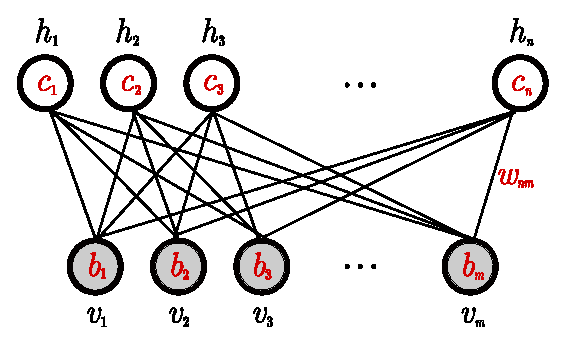
\includegraphics[width=0.4\framewidth]{graphics/RBM-mitParametern-dots3.eps}
%%         \vspace{4mm}
%%
%%         \begin{itemize}
%%	    \item can be seen as stochastic neural network\\
%%	    {\footnotesize Hinton and Sejnowiski, Parallel Distributed Processing, pp. 282-317, MIT, 1986}
%%         \end{itemize}
%%
%%     \end{frame}
%%
%%
%%
%%     \begin{frame}[toc=,bm=]{Restricted Boltzmann Machines (RBMs)}
%%        \vspace{4mm}
%%
%%	 An RBM is an undirected graphical model
%%  
%%         \vspace{4mm}
%%	 \hspace{30mm}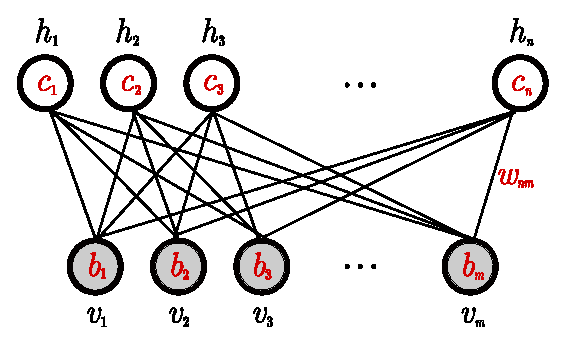
\includegraphics[width=0.4\framewidth]{graphics/RBM-mitParametern-dots3.eps}
%%         \vspace{4mm}
%%
%%         \begin{itemize}
%%	    \item can be seen as stochastic neural network \\
%%	    {\footnotesize Hinton and Sejnowiski, Parallel Distributed Processing, pp. 282-317, MIT, 1986}
%%	    \vspace{2mm}
%%	    \item building block of deep neural networks (Deep Belief Networks) \\
%%	    {\footnotesize Hinton and Salakhutdinov, Science 313, 2006}
%%         \end{itemize}
%%
%%     \end{frame}
%
%     \begin{frame}
%     \frametitle{RBMs can be used ...}
%       \vspace{4mm}
%
%	 ... as \textbf{generative model} of distribution underlying the training data.
%  
%         \vspace{8mm}
%	 \hspace{0.8cm}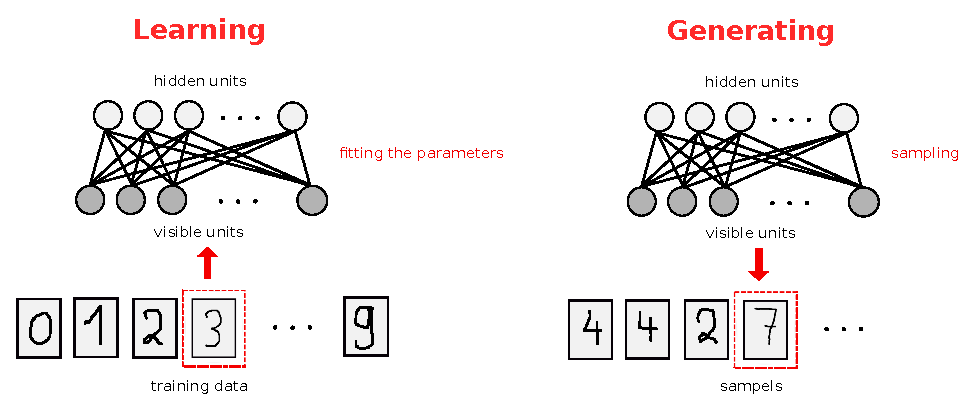
\includegraphics[width=0.9\framewidth]{graphics/rbms1}
%       \vspace{4mm}
%     
%     \end{frame}
% 
% 
%      \begin{frame}
%      \frametitle{RBMs can be used ...}
%       \vspace{4mm}
%
%	 ... as a generative model \textbf{for classification}.
%  
%         \vspace{8mm}
%	 \hspace{0.8cm}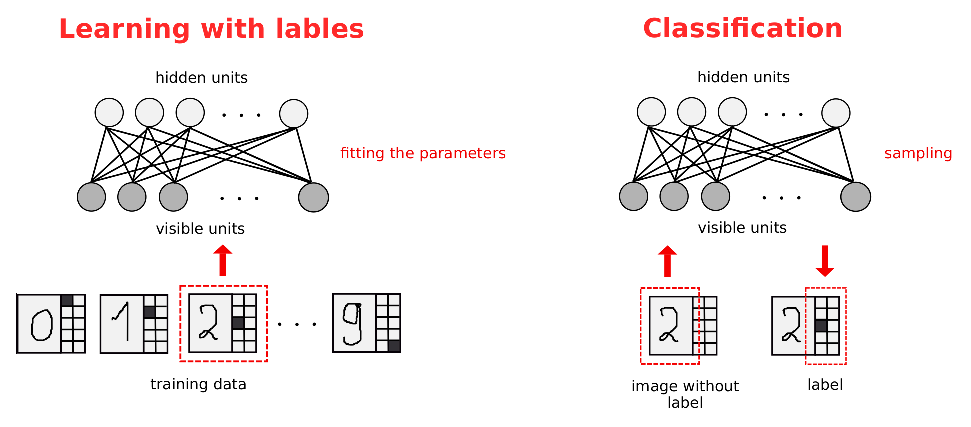
\includegraphics[width=0.9\framewidth]{graphics/rbms3}
%       \vspace{4mm}
%     
%     \end{frame}
% 
% 
%     \begin{frame}
%     \frametitle{RBMs can be used ...}
%       \vspace{1mm}
%
%	 ... as \textbf{feature extractors}.
%  
%	   \vspace{3mm}
%
%        \begin{minipage}{0.45\framewidth}
%%             \centering
%
%	  %\vspace{4mm}
%\begin{figure}
%	     	 %\hspace*{20mm}
%             %\hspace{-1.5cm}
%             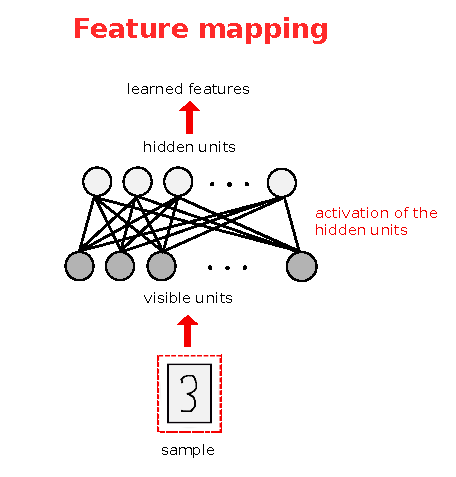
\includegraphics[width=0.4\framewidth]{graphics/rbms2}
%			 
%\end{figure}
%        \end{minipage}    
%        \pause
%\hspace{0.3cm}  \begin{minipage}{0.50\framewidth}
%   \begin{itemize}
%   \item With less hidden than visible neurons this leads to dimensionality reduction.
%   \item Features can serve as input for another learning system.
% %  \item e.g. another RBM which leads to \textbf{deep belief networks}
%  % that can be used as generative models or for unsupervised pretraining of feet forward neural networks.
%  % {\footnotesize [Hinton and Salakhutdinov, Science 313, 2006]}
%   \end{itemize}
%      \end{minipage} 
%     
%     \end{frame}
% 
%    
%\frame
%{
%\frametitle{Conntection to neural networks} 
%
%Todo: Conditional distribution is the sigmoid! (Christians Slides)
%
%}
%
%
%     \begin{frame}
%     \frametitle{RBM-Parameter Fitting}
% 
%         \textbf{Log-likelihood} of model parameters $\vec \theta$ given a training example $\vec x_s$ is
%       %   \vspace{-5mm}
%           \begin{equation*}
%		\ell(\vec \theta|\vec x_s)=  \log p(\vec x_s) 
%		= \log \sum\limits_{ {\vec h}}  e^{-\mathcal{E}(\vec x_s,\vec h)} - \log \sum\limits_{ \vec x, \vec h}  e^{-\mathcal{E}(\vec x,\vec h)}  \enspace.
%	  \end{equation*}
% 
%      \pause
%
%	  \vspace{-2mm}
%	  \textbf{Log-likelihood gradient} is given by:
%	 \begin{align*}
%		\frac{\partial \ell(\vec \theta|\vec x_s)}{\partial \vec \theta} &=
%		-\!\!\sum\limits_{\vec h} p(\vec h|\vec x_s)\frac{\partial \mathcal{E}(\vec x_s,\vec h)}{\partial \vec \theta} 
%		+ \color{red}{\!\!\sum\limits_{\vec x} p(\vec x) \sum\limits_{\vec h} p(\vec h|\vec x) \frac{\partial\mathcal{E} (\vec x, \vec h)}{\partial \vec \theta} } \\% \enspace.
%		&= - \mathbb{E}_{p(\vec h| \vec x_s)}\Big[\frac{\partial \mathcal{E}(\vec x_s,\vec h)}{\partial \vec \theta}  \Big] + \color{red}{\mathbb{E}_{p(\vec h, \vec x)}\Big[\frac{\partial \mathcal{E}(\vec x,\vec h)}{\partial \vec \theta}  \Big]} \enspace\color{black}{.}
%	%	&\approx - \big\langle \frac{\partial \mathcal{E}(\vec x_s,\vec h)}{\partial \vec \theta}  \big\rangle_d + \color{red}{\big\langle \frac{\partial \mathcal{E}(\vec x_s,\vec h)}{\partial \vec \theta}  \big\rangle_m} \enspace\color{black}{.}
%	  \end{align*}
%
%	\pause	  
%	  
%	  \vspace{-0.4cm}
%	  But
%	  \begin{itemize}
%	  \item the second term is intractable for regular sized RBMs.
%	  % because its complexity is exponential in the size of the smallest layer.
%	  \item obtaining (almost) unbiased estimates by MCMC methods typically requires many sampling steps.
%	        $\rightarrow$ Computational effort is too large.
%	  \end{itemize}
%     \end{frame}
%
%
%
%\begin{frame}
%\frametitle{Gibbs Sampling based Learning Algorithms}
%	\textbf{$\pmb{k}$-step Contrastive Divergence (CD-$\pmb{k}$)}
%
%	 \vspace{2mm}
%	  Starting from training example $\vec x^{(0)}$ a Gibbs chain is only run for $k$ steps:  
%	  $\vec x^{(0)} \rightarrow \vec h^{(0)} \rightarrow \vec x^{(1)} \rightarrow \vec h^{(1)} \rightarrow ... \rightarrow \vec x^{(k)}$ .
%	  \pause
%	 
%	 \vspace{2mm}
%	 % Biased ${k}$-step Contrastive Divergence approximation of the log-likelihood gradient is given by:
%	 Log-likelihood gradient is approximated based on $\vec x^{(k)}$ by:
%	 % \only<2>{ 
%	  \begin{align*}
%%	  \operatorname{CD}_k(\vec\theta, \vec x^{(0)}) = &
%	  - \sum\limits_{\vec h} p(\vec h|\vec x^{(0)}) \frac{\partial \mathcal{E}(\vec x^{(0)},\vec h)}{\partial \vec\theta }  
%	    \only<2>{+\color{red}{\!\!\sum\limits_{\vec x} p(\vec x) \sum\limits_{\vec h} p(\vec h|\vec x) \frac{\partial\mathcal{E} (\vec x, \vec h)}{\partial \vec \theta} }  }
%	 \only<3->{+ %\color{white}{\sum\limits_{\vec x} p(\vec x)}
%	 \color{red}{\sum\limits_{\vec h} p(\vec h| \vec x^{(k)})  \frac{\partial \mathcal{E}(\vec x^{(k)}, \vec h)}{\partial \vec\theta }}\enspace\enspace \enspace \color{black}}
%	\end{align*}
%%	  {\footnotesize [Hinton, Osindero \& Teh, Neural Computation 18, 2006]}	  % }
%	  \pause	
%%	  \pause
%	  
%	  
%%	   \vspace{1cm}
%	   
%%	  \begin{block}\Large\centering 
%  %  \textbf{How does the bias influence the learning process?}
%%	 \end{block}


%	 \textbf{Refined variants} 
%
%	  \vspace{-2mm}
%	  \begin{itemize}
%	  \item Persistent Contrastive Divergence (PCD) \\
%	  {\footnotesize [Tieleman, ICML, 2008]} 
%	  \item Fast Persistent Contrastive Divergence (FPCD)\\
%	  {\footnotesize [Tieleman and Hinton, ICML, 2009]} 
%	  \end{itemize}

%     \end{frame}


%\begin{frame}[toc=,bm=]{Gibbs sampling based learning algorithms}
%  \begin{itemize}
%	  \item CD-, PCD- and FPCD-approximations are biased 
%	  \vspace{4mm}
%	  \item bias depends on the mixing rate of the Markov chain 
%	  \vspace{4mm}
%          \item mixing slows down with increasing absolute values of model parameters 
%	  \end{itemize}
%
%\end{frame}


%%\setcounter{famenumber}{15}
%\begin{frame}
%\frametitle{Gibbs sampling based learning algorithms}
%  \begin{itemize}
%	  \item CD-, PCD- and FPCD-approximations are biased.
%	  \vspace{4mm}
%	  \item Bias depends on mixing rate of the Markov chain. 
%	  \vspace{4mm}
%      \item Mixing slows down with increasing absolute values of RBM parameters.
%	  \end{itemize}
%
%	 \pause
%
%	 \vspace{1cm}
%	 \begin{block}\Large\centering 
%	 How does the bias influence the learning process?
%	 \end{block}
%
%\end{frame}

 
 




%\begin{frame}
%\frametitle{Divergence of CD-learning}
%    
%    \only<1>{
%    
%    \begin{block}\Large\centering 
%We found that the approximation error can distort the learning process.
%{\footnotesize [Fischer \& Igel, ICANN, 2010]}
%\end{block}
%
%   \vspace{0.2cm}
%   Log-likelihood during training small RBMs 
%    with CD-$k$ on artificial data sets.
%    
%   % \pause
%
%     %\vspace{1mm}
%	%\begin{itemize}
%	%\item For \textbf{different choices of $k$}:
%	%\end{itemize}
%
%    %\psfrag{k=1}[l][l]{{\fontsize{1}{12} \selectfont$k=1$}}
%    %\psfrag{k=2}[l][l]{{\fontsize{1}{12} \selectfont$k=2$}}
%    %\psfrag{k=4}[l][l]{{\fontsize{1}{12} \selectfont$k=4$}}
%    %\psfrag{k=10}[l][l]{{\fontsize{1}{12} \selectfont$k\!=\!10$}}
%    %\psfrag{k=100}[l][l]{{\fontsize{1}{12} \selectfont$k\!=\!100$}}
%	\psfrag{iterations}[b][t]{\tiny iterations}
%	\psfrag{iterationen}[b][t]{\tiny iterations}
%	\psfrag{log-likelihood}[bt][t]{\tiny log-likelihood}
%	\psfrag{shifter}[bt][t]{\tiny \textbf{Shifter}}
%	\psfrag{bas}[bt][t]{\tiny \textbf{Bars-and-Stripes}}
%
%
%   % \hspace{-4mm}
%    %\includegraphics[width=0.9\columnwidth]{Shifter_k_aistats.eps}
%   % \hspace{-8mm} \includegraphics[width=0.52\columnwidth]{%BAS_k_aistats.eps}
%	
%	%  \vspace{-15mm}
%	\parbox{\textwidth}{\hspace{3cm}\includegraphics[width=.8\textwidth]{help.eps}}%\hspace{-0.7 cm}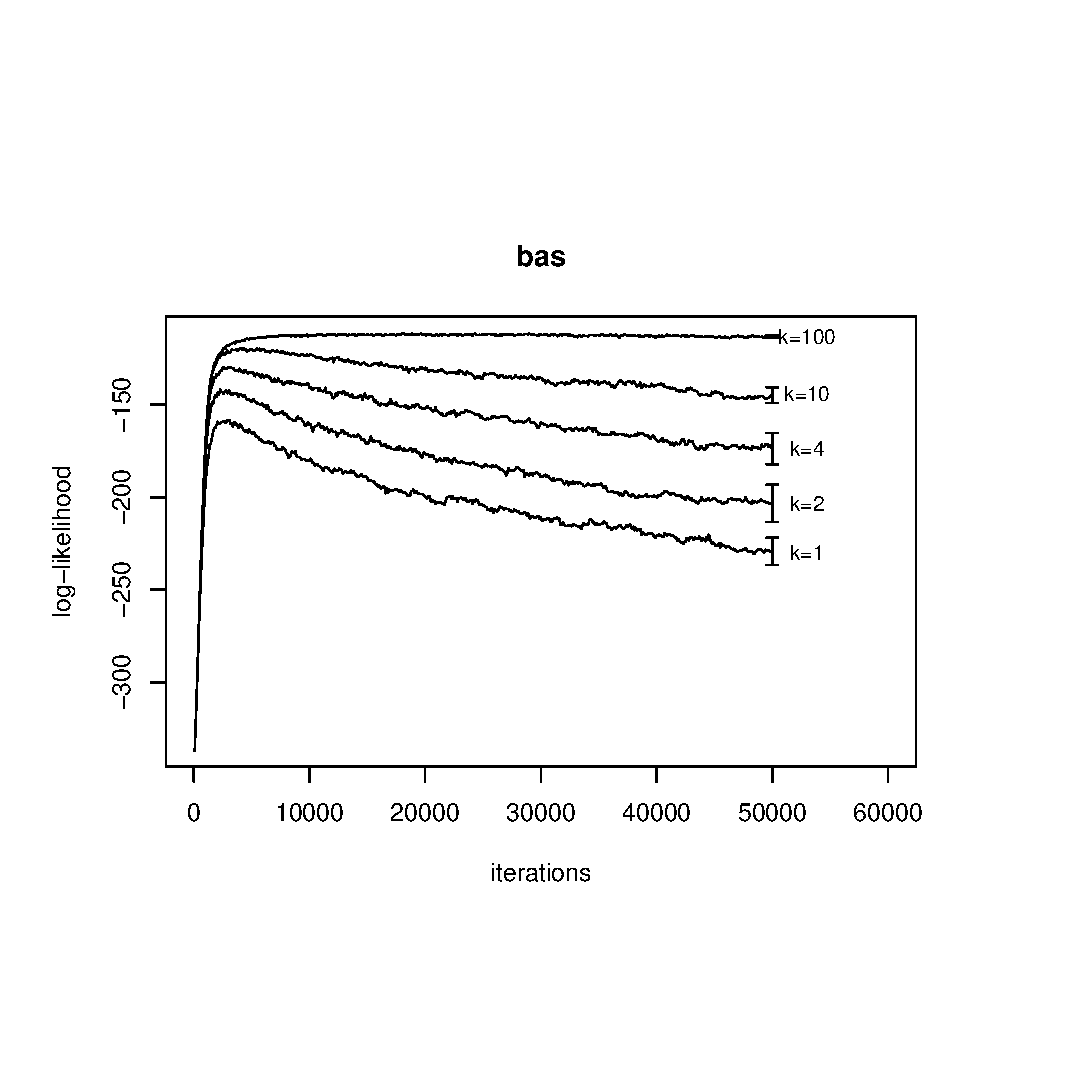
\includegraphics[width=.53\textwidth]{graphics/BAS_k_ICANN_t}}
%%	\parbox{1\textwidth}{\hspace{1cm}\includegraphics[]{help.eps}}
%   %  \vspace{-10mm}
% 
%     %   \vspace{-1cm}\hspace{3mm} 	
% 	%\footnotesize [Fischer \& Igel, ICANN, 2010]}
% 	%\pause
% 	  %\vspace{-2cm}
%% 	  \only<2>{
%% 	  % \vspace{-1cm}
%%    We analyzed the log-likelihood during training small RBMs 
%%    with CD-$k$ on artificial benchmark sets.
%%    
%%   % \pause
%%
%%     %\vspace{1mm}
%%	\begin{itemize}
%%	\item For \textbf{different choices of $k$}:
%%	\end{itemize}
%%
%%    %\psfrag{k=1}[l][l]{{\fontsize{1}{12} \selectfont$k=1$}}
%%    %\psfrag{k=2}[l][l]{{\fontsize{1}{12} \selectfont$k=2$}}
%%    %\psfrag{k=4}[l][l]{{\fontsize{1}{12} \selectfont$k=4$}}
%%    %\psfrag{k=10}[l][l]{{\fontsize{1}{12} \selectfont$k\!=\!10$}}
%%    %\psfrag{k=100}[l][l]{{\fontsize{1}{12} \selectfont$k\!=\!100$}}
%%	\psfrag{iterations}[b][t]{\tiny iterations}
%%	\psfrag{iterationen}[b][t]{\tiny iterations}
%%	\psfrag{log-likelihood}[bt][t]{\tiny log-likelihood}
%%	\psfrag{shifter}[bt][t]{\tiny \textbf{Shifter}}
%%	\psfrag{bas}[bt][t]{\tiny \textbf{Bars-and-Stripes}}
%%
%%
%%   % \hspace{-4mm}
%%    %\includegraphics[width=0.9\columnwidth]{Shifter_k_aistats.eps}
%%   % \hspace{-8mm} \includegraphics[width=0.52\columnwidth]{%BAS_k_aistats.eps}
%%	
%%	%  \vspace{-15mm}
%%	\parbox{\textwidth}{\hspace{3cm}\includegraphics[width=.8\textwidth]{help.eps}}%\hspace{-0.7 cm}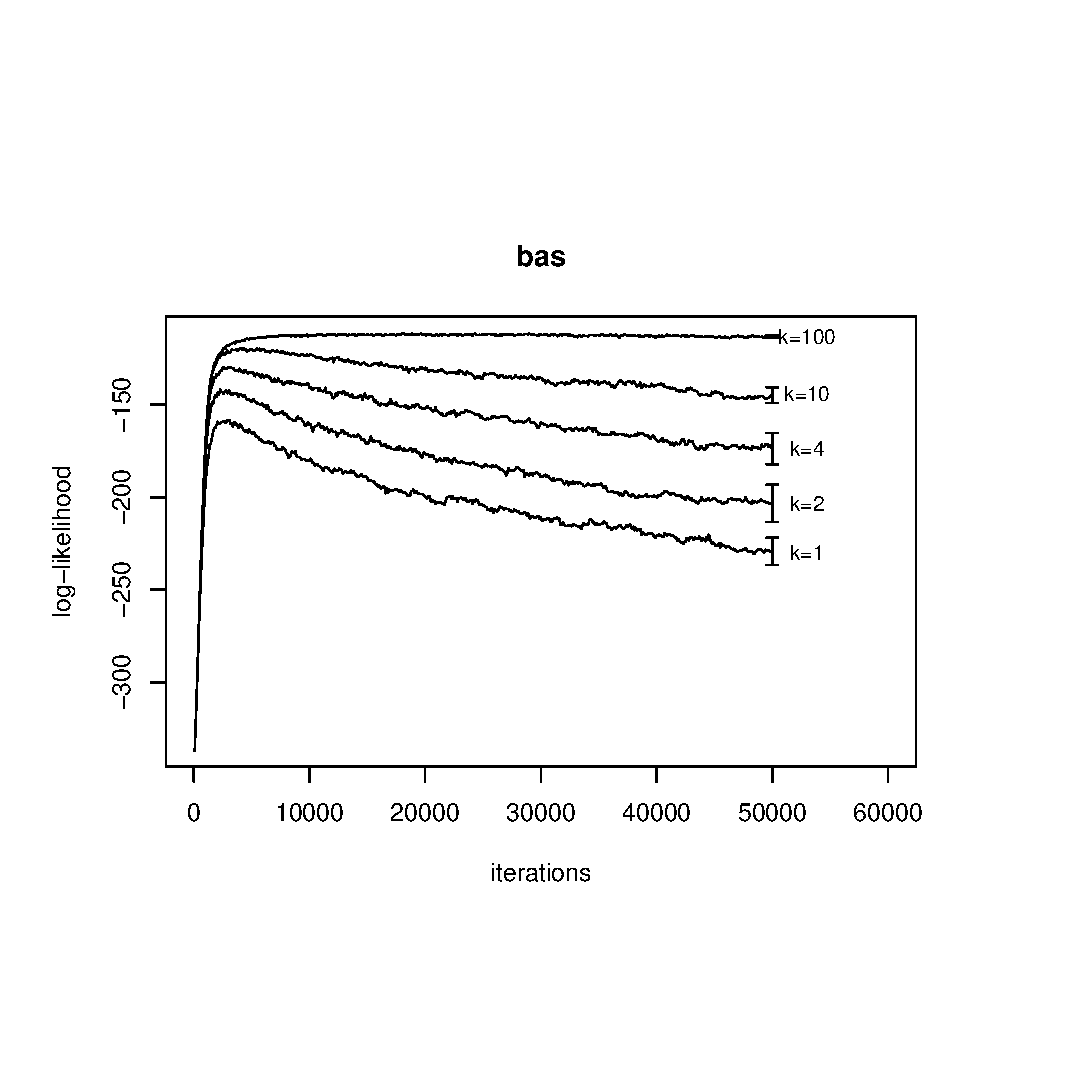
\includegraphics[width=.53\textwidth]{graphics/BAS_k_ICANN_t}}
%%%	\parbox{1\textwidth}{\hspace{1cm}\includegraphics[]{help.eps}}
%%   %  \vspace{-10mm}
%% 
%%    %    \vspace{-2cm}\
%% 	% \begin{block}\Large\centering 
%%\textbf{Can we get an theoretical estimate of the bias of CD?}
%%	% \end{block}
%%	}}
%   }
%   \end{frame}


   
%   \begin{frame}[toc=,bm=]{Experiments}
%
%    log-likelihood for CD-$k$ with different choices of $k$
%
%    \psfrag{k=1}[l][l]{\tiny\tiny$k\!=\!1$}
%    \psfrag{k=2}[l][l]{\tiny$k\!=\!2$}
%    \psfrag{k=4}[l][l]{\tiny$k\!=\!4$}
%    \psfrag{k=10}[l][l]{\tiny$k\!=\!10$}
%    \psfrag{k=100}[l][l]{\tiny$k\!=\!100$}
%	\psfrag{iterations}[b][t]{\tiny iterations}
%	\psfrag{iterationen}[b][t]{\tiny iterations}
%	\psfrag{log-likelihood}[bt][t]{\tiny log-likelihood}
%	\psfrag{shifter}[bt][t]{\tiny \textbf{Shifter}}
%	\psfrag{bas}[bt][t]{\tiny \textbf{Bars-and-Stripes}}
%
%    \vspace{-10mm}
%    \hspace{8mm}
%    %\includegraphics[width=0.9\columnwidth]{Shifter_k_aistats.eps}
%    %\hspace{-8mm} \includegraphics[width=0.52\columnwidth]{BAS_k_aistats.eps}
%	
%	\parbox{\textwidth}{\includegraphics[width=.5\textwidth]{graphics/Shifter_k_ICANN_t}\hspace{-0.7 cm}\includegraphics[width=.5\textwidth]{graphics/BAS_k_ICANN_t}}
%    
% \vspace{-10mm}
%     \begin{itemize}
%	  \item a \underline{good} schedule for increasing $k$ could solve the problem
%     \end{itemize}
% 
%   \end{frame}

 

%    \begin{frame}
%    \frametitle{Divergence of CD-learning}
%  
%    \vspace{2mm}
%    We analyzed the log-likelihood during training small RBMs 
%    with CD-$k$ on artificial benchmark sets.
%
%%    \pause
%%
%%    \vspace{1mm}
%%	\begin{itemize}
%%	\item For CD-$1$ and weight-decay with \textbf{different choices of weight decay parameter $\lambda$}:
%%	\end{itemize}
%
%
%    \psfrag{0.05}[l][l][.9]{{\fontsize{1}{12} \selectfont $0.05$}}
% 	\psfrag{0.00005}[l][l][.9]{{\fontsize{1}{12} \selectfont$5\cdot10^{-5}$}}
% 	\psfrag{0.0005}[l][l][.9]{{\fontsize{1}{12} \selectfont$0.0005$}}
% 	\psfrag{wd=0.005}[lb][lt][.9]{{\fontsize{1}{12} \selectfont$0.005$}}
% 	\psfrag{wd=5e-05}[l][l][.9]{{\fontsize{1}{12} \selectfont$5\cdot10^{-5}$}}%{\tiny$\lambda\!=\!0.00005$}
% 	\psfrag{wd=0.0005}[l][l][.9]{{\fontsize{1}{12} \selectfont$5\cdot10^{-4}$}}
%	\psfrag{iterations}[b][t]{\tiny iterations}
%	\psfrag{log-likelihood}[bt][t]{\tiny log-likelihood}
%	\psfrag{shifter}[bt][t]{\tiny \textbf{Shifter}}
%	\psfrag{bas}[bt][t]{\tiny \textbf{Bars-and-Stripes}}
%
%   % \vspace{-0.4cm}
%    %\hspace{-4mm}
%    %\includegraphics[width=0.9\columnwidth]{Shifter_wd_aistats.eps}
%    % \hspace{-8mm} \includegraphics[width=0.52\columnwidth]{BAS_wd_aistats.eps}
%	%\parbox{1\textwidth}{\includegraphics[width=.53\framewidth]{graphics/Shifter_wd_ICANN_t}\hspace{-0.7 cm}\includegraphics[width=.53\framewidth]{graphics/BAS_wd_ICANN_t}}
%	%\parbox{1\textwidth}{\hspace{1cm}\includegraphics[framewidth]{help2}}
%
%     %\vspace{-10mm}
%    
% \end{frame}
%
%
%%\begin{frame}[toc=,bm=]{Experiments}
%%
%%    log-likelihood for CD-$1$ and weight-decay with different choices of $\lambda$
%%	  \psfrag{0.05}[l][l][.9]{\tiny$\lambda\!=\!0.05$}
%% 	\psfrag{0.00005}[l][l][.9]{\tiny$\lambda\!=\!5\cdot10^{-5}$}
%% 	\psfrag{0.0005}[l][l][.9]{\tiny$\lambda\!=\!0.0005$}
%% 	\psfrag{wd=0.005}[lb][lt][.9]{\tiny$\lambda\!=\!0.005$}
%% 	\psfrag{wd=5e-05}[l][l][.9]{\tiny$\lambda\!=\!5\cdot10^{-5}$}%{\tiny$\lambda\!=\!0.00005$}
%% 	\psfrag{wd=0.0005}[l][l][.9]{\tiny$\lambda\!=\!5\cdot10^{-4}$}
%%	\psfrag{iterations}[b][t]{\tiny iterations}
%%	\psfrag{log-likelihood}[bt][t]{\tiny log-likelihood}
%%	\psfrag{shifter}[bt][t]{\tiny \textbf{Shifter}}
%%	\psfrag{bas}[bt][t]{\tiny \textbf{Bars-and-Stripes}}
%%
%%    \vspace{-10mm}
%%    \hspace{8mm}
%%    %\includegraphics[width=0.9\columnwidth]{Shifter_wd_aistats.eps}
%%    % \hspace{-8mm} \includegraphics[width=0.52\columnwidth]{BAS_wd_aistats.eps}
%%	\parbox{\textwidth}{\includegraphics[width=.5\textwidth]{graphics/Shifter_wd_ICANN_t}\hspace{-0.7 cm}\includegraphics[width=.5\textwidth]{graphics/BAS_wd_ICANN_t}}
%%
%%     \vspace{-10mm}
%%     \begin{itemize}
%%	  \item the \underline{right} weight-decay parameter could solve the problem
%%     \end{itemize}
%%
%%    \end{frame}



%\begin{frame}[toc=,bm=]{Experiments}
%
%    log-likelihood for CD-$1$ in RBMs with different numbers of hidden neurons
%	  
%    \psfrag{n=19}[l][l]{\!\tiny$n\!=\!19$}
%	\psfrag{n=10}[l][l]{\!\tiny$n\!=\!10$}
%	\psfrag{n=38}[l][l]{\!\tiny$n\!=\!38$}
%	\psfrag{h=8}[l][l]{\!\tiny$n\!=\!8$}
%	\psfrag{h=16}[l][l]{\!\tiny$n\!=\!16$}
%	\psfrag{h=32}[l][l]{\!\tiny$n\!=\!32$}
%	\psfrag{iterations}[b][t]{\tiny iterations}
%	\psfrag{iteratios}[b][t]{\tiny iterations}
%	\psfrag{log-likelihood}[bt][t]{\tiny log-likelihood}
%	\psfrag{shifter}[bt][t]{\tiny \textbf{Shifter}}
%	\psfrag{bas}[bt][t]{\tiny \textbf{Bars-and-Stripes}}
%
%    \vspace{-10mm}
%    \hspace{8mm}
%    %\includegraphics[width=0.9\columnwidth]{Shifter_wd_aistats.eps}
%    % \hspace{-8mm} \includegraphics[width=0.52\columnwidth]{BAS_wd_aistats.eps}
%	\parbox{\textwidth}{\includegraphics[width=.5\textwidth]{graphics/Shifter_nh_ICANN_t}\hspace{-0.7 cm}\includegraphics[width=.5\textwidth]{graphics/BAS_nh_ICANN_t}}
%
%    \vspace{-10mm}
%
% \end{frame}
%
%
%\begin{frame}[toc=,bm=]{Experiments}
%
%    log-likelihood for CD-$1$ in RBMs with different numbers of hidden neurons
%	  
% 	\psfrag{n=19}[l][l]{\!\tiny$n\!=\!19$}
%	\psfrag{n=10}[l][l]{\!\tiny$n\!=\!10$}
%	\psfrag{n=38}[l][l]{\!\tiny$n\!=\!38$}
%	\psfrag{h=8}[l][l]{\!\tiny$n\!=\!8$}
%	\psfrag{h=16}[l][l]{\!\tiny$n\!=\!16$}
%	\psfrag{h=32}[l][l]{\!\tiny$n\!=\!32$}
%	\psfrag{iterations}[b][t]{\tiny iterations}
%	\psfrag{iteratios}[b][t]{\tiny iterations}
%	\psfrag{log-likelihood}[bt][t]{\tiny log-likelihood}
%	\psfrag{shifter}[bt][t]{\tiny \textbf{Shifter}}
%	\psfrag{bas}[bt][t]{\tiny \textbf{Bars-and-Stripes}}
%
% 	\vspace{-10mm}
%    \hspace{8mm}
%    %\includegraphics[width=0.9\columnwidth]{Shifter_wd_aistats.eps}
%    % \hspace{-8mm} \includegraphics[width=0.52\columnwidth]{BAS_wd_aistats.eps}
%	\parbox{\textwidth}{\includegraphics[width=.5\textwidth]{graphics/Shifter_nh_ICANN_t}\hspace{-0.7 cm}\includegraphics[width=.5\textwidth]{graphics/BAS_nh_ICANN_t}}
%
%    \vspace{-10mm}
%
%    \begin{itemize}
%	  \item divergence seems to occur especially in the case of target distributions that are difficult to learn
%    \end{itemize}
%    
% \end{frame}





%\begin{frame}[toc=,bm=]{Future Work}
%  
%	\begin{itemize}
%	    \item finding a stopping criterion
%	    \vspace{4mm}
%	    \item finding a heuristic for the weight-decay parameter
%	    \vspace{4mm}
%	    \item analyzing learning and scaling behavior of algorithms based on tempered transitions  
%
%	    (\footnotesize Salakhutdinov, NIPS, 2009; Desjardins et al., AISTATS, 2010)
%	\end{itemize}
%      
%\end{frame}


%\subsection{Bounding the bias of CD}

%  \begin{frame}
%  \frametitle{Bounding the Bias of CD}
%      %\begin{theorem}
%    
%  \vspace{-3mm}
%  \begin{block}\Large\centering 
%We derived a upper bound for the approximation error. \\
%{\footnotesize [Fischer \& Igel, Neural Computation, 2011]}
%\end{block}
%      
%      \textbf{Theorem.}
%      Given an RBM with $m$ visible and $n$  hidden variables and joint probability
%      distribution $p$. 
%      Let $p_e$ be the empirical distribution defined
%      by a set of samples $\vec x_1,\dots,\vec x_\ell$.  Then an upper
%      bound on the expectation of the error of the CD-$k$ approximation of
%      the {log-likelihood} derivative w.r.t. some RBM parameter $\theta$ is given by
%      \only<1>{
%      \hspace{-5cm}\begin{multline*}
%       \left| E_{p_e(\vec x^{(0)})}\left[E_{p(\vec x^{(k)}|\vec
%       x^{(0)})}\left[\frac{\partial \log p(\vec x^{(k)})}{\partial
%       \theta} \right]\right]\right| 
%       \leq \frac{1}{2} \color{black}{\left|\mu - p\right|}\color{black}{\left(1-e^{-(m+n) \Delta}\right)^k}
%      \end{multline*}
%      with 
%      %$m$ and $n$ being the number of visible and hidden neurons respectively, 
%      $\Delta$ being the maximum change in energy caused by changing the value of one single variable 
%      and a start distribution $\mu(\vec x, \vec h )= p(\vec h|\vec x) p_e(\vec x) \enspace$
%%      \begin{equation*}
%%      \mu(\vec v, \vec h )= p(\vec h|\vec v) p_e(\vec v) \enspace
%%      \end{equation*}
%      for the initial states of the chain.
%     
%%      \vspace{2mm}
%%       {\footnotesize [Fischer \& Igel, Neural Computation, 2011]}
%} 
%      \pause
%      \only<2>{
%      \begin{multline*}
%       \left| E_{p_e(\vec x^{(0)})}\left[E_{p(\vec x^{(k)}|\vec
%       x^{(0)})}\left[\frac{\partial \log p(\vec x^{(k)})}{\partial
%       \theta} \right]\right]\right| 
%       \leq \frac{1}{2} \color{red}{\left|\mu - p\right|}\color{black}{\left(1-e^{-(m+n) \Delta}\right)}^{\color{black}{k}}
%      \end{multline*}
%      with 
%      %$m$ and $n$ being the number of visible and hidden neurons respectively, 
%      $\Delta$ being the maximum change in energy caused by changing the value of one single variable 
%      and a start distribution $\mu(\vec x, \vec h )= p(\vec x|\vec x) p_e(\vec x) \enspace$
%%      \begin{equation*}
%%      \mu(\vec v, \vec h )= p(\vec h|\vec v) p_e(\vec v) \enspace
%%      \end{equation*}
%      for the initial states of the chain.
%      
%   %   \vspace{2mm}
%   %    {\footnotesize [Fischer \& Igel, Neural Computation, 2011]}
%   }
%      \pause
%      \only<3>{
%      \begin{multline*}
%       \left| E_{p_e(\vec x^{(0)})}\left[E_{p(\vec x^{(k)}|\vec
%       x^{(0)})}\left[\frac{\partial \log p(\vec x^{(k)})}{\partial
%       \theta} \right]\right]\right|  
%       \leq \frac{1}{2} \color{black}{\left|\mu - p\right|}\color{black}{\left(1-e^{\color{red}{ -(m+n) \Delta}}\right)}^{\color{black}{k}}
%      \end{multline*}
%      with 
%      %$m$ and $n$ being the number of visible and hidden neurons respectively, 
%      $\Delta$ being the maximum change in energy caused by changing the value of one single variable 
%      and a start distribution $\mu(\vec x, \vec h )= p(\vec h|\vec x) p_e(\vec x) \enspace$
%%      \begin{equation*}
%%      \mu(\vec v, \vec h )= p(\vec h|\vec v) p_e(\vec v) \enspace
%%      \end{equation*}
%      for the initial states of the chain.
%      
%%      \vspace{2mm}
%%      {\footnotesize [Fischer \& Igel, Neural Computation, 2011]}
%}
%\pause
% \only<4>{
%      \begin{multline*}
%       \left| E_{p_e(\vec x^{(0)})}\left[E_{p(\vec x^{(k)}|\vec
%       x^{(0)})}\left[\frac{\partial \log p(\vec x^{(k)})}{\partial
%       \theta} \right]\right]\right|  
%       \leq \frac{1}{2} \color{black}{\left|\mu - p\right|}\color{black}{\left(1-e^{\color{black}{ -(m+n) \Delta}}\right)}^{\color{red}{k}}
%      \end{multline*}
%      with 
%      %$m$ and $n$ being the number of visible and hidden neurons respectively, 
%      $\Delta$ being the maximum change in energy caused by changing the value of one single variable 
%      and a start distribution $\mu(\vec x, \vec h )= p(\vec h|\vec x) p_e(\vec x) \enspace$
%%      \begin{equation*}
%%      \mu(\vec v, \vec h )= p(\vec h|\vec v) p_e(\vec v) \enspace
%%      \end{equation*}
%      for the initial states of the chain.
%     
%       }
%      %\end{theorem}
%     \end{frame}

%\begin{frame}
%\frametitle{Bias and bound}
%
%\vspace{0.5cm}
%\includegraphics[width=0.9\columnwidth]{graphics/NECO-05-10-1248-Figure.eps} 
%
%\pause 
%%Bound is closely related to bound on mixing rate of Gibbs sampler.
% \vspace{1cm}
%\begin{block}\Large\centering 
%	 Can we increase mixing for sampling from RBMs ?
%	 \end{block}
%\end{frame} 

%\begin{frame}
%\frametitle{Improvements for RBM Training}
%
%We improved training by 
% 
%\begin{block}\Large\centering 	 
%proposing a new transition operator for faster mixing in RBMs.\\
%{\footnotesize [Br\"ugge, Fischer \& Igel, Machine Learning, 2013]}
% \end{block}
%  
%  \pause
%\begin{block}\Large\centering 	 
%proposing a consistent estimate of the likelihood gradient.\\
%{\footnotesize [Krause, Fischer \& Igel, Pattern Recognition Letters, 2018]}
% \end{block}
%
%
% \pause
% \begin{block}\Large\centering 	
%investigating a different parametrization of RBMs and deep BMs. \\
%{\footnotesize [Melchior, Fischer \& Wiskott, JMLR, 2016]}
%\end{block}
%
%\pause
%\begin{block}\Large\centering 
%	investigating Banneth's acceptance ratio and other estimates of the normalization constant. \\
%{\footnotesize [Krause, Fischer \& Igel, submitted]}
% \end{block}
% 
% 
%\end{frame} 
%
%\begin{frame}
%\frametitle{Analysis of RBMs and their Training Algorithms}
% We continued our theoretical analysis by 
% 
%%\begin{block}\Large\centering 
%%	 analyzing RBM  training based on the sign of the gradient approximations.\\ {\footnotesize [Fischer \& Igel, ESANN, 2011]}
%%	 \end{block}
%
%% \pause
%\begin{block}\Large\centering 	 
%analyzing the approximation properties of deep belief networks with real-valued visible and binary hidden variables.\\
%{\footnotesize [Krause, Fischer, Glasmachers \& Igel, ICML, 2013]}
% \end{block}
% 
% \pause 
%  \begin{block}\Large\centering 	 
%deriving a lower bound for the convergence rate of parallel tempering for sampling RBMs.\\
%{\footnotesize [Fischer \& Igel, Theoretical Computer Science, 2015]}
% \end{block}
% 
%%  \pause
%% \begin{block}\Large\centering 	 
%% writing an introductory paper to RBMs anf their training methods.\\
%%{\footnotesize [Fischer \& Igel, Pattern Recognition, 2014]}
%% \end{block}
%
% \end{frame} 
%


%\subsection{Variational Autoencoder}


%\frame{\frametitle{Outline}\tableofcontents}
 %\AtBeginSubsection[]
% {
%   \begin{frame}
%       \frametitle{Outline}
%       %\tableofcontents[currentsection,currentsubsection]
%       \tableofcontents[currentsection]
%   \end{frame}
% }
% 

\section{Directed generative models}


 \frame{
\frametitle{Directed generative models}

Learn to generate $\vec x$ from some latent variables $\vec z$.

$$p_{\vec \theta}(\vec x) = \int p_{\vec \theta}(\vec x, \vec z) d\vec z = \int p_{\vec \theta}(\vec x| \vec z) p_{\vec \theta}(\vec z) d\vec z$$

%Todo: h zu z machen, theta einbauen moeglich?!!!
\begin{figure} 
%\hspace{-3cm}
\includegraphics[width=4cm]{VAE.png}
\includegraphics[width=7cm]{zToxManifold.png}
\end{figure}

\tiny{Image from: Ward, A. D., Hamarneh, G.: \textbf{3D Surface Parameterization Using Manifold Learning for Medial Shape Representation}, Conference on Image Processing, Proc. of SPIE Medical Imaging, 2007}

}

 \frame{
\frametitle{Directed generative models}

The classic DAG problem: Where does $\vec z$ come from?

\begin{itemize}
\item %For inference we need 
The posterior  is given by $p_{\vec \theta}(\vec z| \vec x ) = \frac{p_{\vec \theta}(\vec x| \vec z)p_{\vec \theta}(\vec z)}{p_{\vec \theta}(\vec x)}$.
%
\pause
\item But $p_{\vec \theta}(\vec x)=\int p_{\vec \theta}(\vec x|\vec z) p_{\vec \theta}(\vec z) d\vec z$ is intractable.
\end{itemize}

%An VAE contains two directed graphical models
%An VAE  consists of directed graphical models

%\vspace{0.7cm}
%\only<1-3>{\hspace{2,3cm
\hspace{5.4cm}\includegraphics[width=0.37\framewidth]{VAE.png}

We will see two approaches to this problems:
\begin{itemize}
\item Variational Autoencoders (VAEs)
\item Generative Adversarial Networks (GANs)
\end{itemize}

}



\section{Variational Autoencoder (VAE)}


 \begin{frame}
\frametitle{Variational Autoencoder (VAE)}

The classic DAG problem: Where does $\vec z$ come from?

Idea: introduce an \textbf{inference model $q_{\vec \phi }(\vec z| \vec x)$}  that learns to approximate the posterior   $p_{\vec \theta}(\vec z| \vec x )$

\hspace{1.5cm}\includegraphics[width=0.7\framewidth]{VAE-full.png}


Independently proposed by:
\begin{itemize}
\item Kingma and Welling, \emph{Auto-Encoding Variational Bayes}, ICLR 2014
\item Rezende, Mohamed and Wierstra, \emph{Stochastic back-propagation and variational inference in deep latent Gaussian models.} ICML 2014
\end{itemize}

%\begin{itemize}
%\item To do inference one would like to calculate $p(\vec z| \vec x ) = \frac{p(\vec x| \vec z)p(\vec z)}{p(\vec x)}$.
%
%\pause
%\item But $p_{\vec \theta}(\vec x)=\int p_{\vec \theta}(\vec x|\vec z) p_{\vec \theta}(\vec z) d\vec z$ is intractable.
%\end{itemize}

%An VAE contains two directed graphical models
%An VAE  consists of directed graphical models

%\vspace{0.7cm}
%\only<1-3>{
%\hspace{2,3cm} 
%\includegraphics[width=0.7\framewidth]{VAE}
%\vspace{0.7cm}
%with distributions
%with distribution
%\vspace{-0.4cm}
%\begin{align}
% p(\xVec, \hVec)  &= p(\xVec|\hVec_1) p(\hVec_1|\hVec_2) ... p(\hVec_L) \nonumber 
%\end{align}
%\pause 
%\vspace{-0.4cm}
%\begin{itemize}
%\item To do inference one would like to calculate $p(\vec h| \vec x ) = \frac{p(\vec x| \vec h)p(\vec h)}{p(\vec x)}$.
%
%\pause
%\item But $p(\vec x)=\int p(\vec x|\vec h) p(\vec h) d\vec h$ is intractable.
%\end{itemize}
%} 
%\only<4>{\hspace{2,3cm} \includegraphics[width=0.7\framewidth]{VAE-full}\\

%with distributions
%\vspace{-0.4cm}
%with distribution
%\begin{align}
% p(\xVec, \hVec)  &= p(\xVec|\hVec) p(\hVec)  \nonumber \\
%q(\hVec | \xVec) &= q(\hVec|\xVec) q(\hVec|\hVec_1) ... %q(\hVec_L | \hVec_{L-1}) \nonumber
% \nonumber
%\end{align}}

%\small{[Kingma and Welling, Auto-Encoding Variational Bayes, ICLR 2014]}

%\small{[Rezende, Mohamed and Wierstra, Stochastic back-propagation and variational inference in deep latent Gaussian models. ICML 2014]}

\end{frame} 


\begin{frame}
\frametitle{VAE-Parameter Fitting: Variational Lower Bound}

%Since $\log p(\vec x_s)$ is intractable, optimization is often based on   
%\textbf{variational lower bound} (or \textbf{Evidence Lower BOund (ELBO)}) 
%\textbf{Evidence Lower BOund (ELBO)}
%of log-likelihood for training example $\vec x_s$
\begin{itemize}
\item $\log p(\vec x)$ is intractable.
\item But we can compute a \textbf{variational lower bound}
%\textbf{Evidence Lower BOund (ELBO)}
\end{itemize}
%\pause 
\only<1>{
\begin{align*}
\log p_{\vec \theta}(\vec x) &= \log\int p_{\vec \theta}(\vec x,\vec z) d\vec z =  \log \int  q_{\vec \phi}(\vec z|\vec x) \frac{p_{\vec \theta}(\vec x,\vec z)}{q_{\vec \phi}(\vec z|\vec x)} d\vec z \\ 
&\color{white}{\geq  \int  q(\vec h|\vec x_s)  \log \frac{p(\vec x_s,\vec h)}{q(\vec h|\vec x_s)} d\vec h }\\
&\color{white}{\geq \int  q(\vec h|\vec x_s)  \big( \log p(\vec x_s|\vec h) + \log p(\vec h) - \log q(\vec h|\vec x_s) \big)d\vec h} \\
& \color{white}{mathbb{E}_{q(\vec h|\vec x_s)}\big[ \log p(\vec x_s|\vec h) \big] - KL\big[ q(\vec h|\vec x_s) ||  p(\vec h) \big] }
\end{align*}}
\only<2>{
\begin{align*}
\log p_{\vec \theta}(\vec x) &= \log\int p_{\vec \theta}(\vec x,\vec z) d\vec z =  \log \int  q_{\vec \phi}(\vec z|\vec x) \frac{p_{\vec \theta}(\vec x,\vec z)}{q_{\vec \phi}(\vec z|\vec x)} d\vec z \\ 
&\color{black}{\geq  \int  q_{\vec \phi}(\vec z|\vec x)  \log \frac{p_{\vec \theta}(\vec x,\vec z)}{q_{\vec \phi}(\vec z|\vec x)} d\vec z }\\
&\color{white}{= \int  q(\vec h|\vec x_s)  \big( \log p(\vec x_s|\vec h) + \log p(\vec h) - \log q(\vec h|\vec x_s) \big)d\vec h} \\
& \color{white}{mathbb{E}_{q(\vec h|\vec x_s)}\big[ \log p(\vec x_s|\vec h) \big] - KL\big[ q(\vec h|\vec x_s) ||  p(\vec h) \big] }
\end{align*}
\begin{block}{Jensen’s inequality}
Let $f$ be a convex function  and $X$ an integrable random variable. Then it holds:
$f(\mathcal{E}[X] \leq \mathcal{E}[f(X)]$.
\end{block}


}
\only<3>{
\begin{align*}
\log p_{\vec \theta}(\vec x) &= \log\int p_{\vec \theta}(\vec x,\vec z) d\vec z =  \log \int  q_{\vec \phi}(\vec z|\vec x) \frac{p_{\vec \theta}(\vec x,\vec z)}{q_{\vec \phi}(\vec z|\vec x)} d\vec z \\ 
&\color{black}{\geq  \int  q_{\vec \phi}(\vec z|\vec x)  \log \frac{p_{\vec \theta}(\vec x,\vec z)}{q_{\vec \phi}(\vec z|\vec x)} d\vec z }\\
%&\color{black}{= \int  q_{\vec \phi}(\vec z|\vec x)  \big( \log p_{\vec \theta}(\vec x|\vec z) + \log p_{\vec \theta}(\vec z) - \log q_{\vec \phi}(\vec z|\vec x) \big)d\vec z} \\
&\color{black}{= \int  q_{\vec \phi}(\vec z|\vec x)  \big( \log p_{\vec \theta}(\vec x|\vec z) + \log \frac{p_{\vec \theta}(\vec z)}{ q_{\vec \phi}(\vec z|\vec x)} \big)d\vec z} \\
& \color{white}{mathbb{E}_{q(\vec h|\vec x_s)}\big[ \log p(\vec x_s|\vec h) \big] - KL\big[ q(\vec h|\vec x_s) ||  p(\vec h) \big] }
\end{align*}
%Todo: Box mit Logarithmus-Regeln einbauen!
}
\only<4>{
\begin{align*}
\log p_{\vec \theta}(\vec x) &= \log\int p_{\vec \theta}(\vec x,\vec z) d\vec z =  \log \int  q_{\vec \phi}(\vec z|\vec x) \frac{p_{\vec \theta}(\vec x,\vec z)}{q_{\vec \phi}(\vec z|\vec x)} d\vec z \\  
&\color{black}{\geq  \int  q_{\vec \phi}(\vec z|\vec x)  \log \frac{p_{\vec \theta}(\vec x,\vec z)}{q_{\vec \phi}(\vec z|\vec x}) d\vec z }\\
&\color{black}{= \int  q_{\vec \phi}(\vec z|\vec x)  \big( \log p_{\vec \theta}(\vec x|\vec z) + \log \frac{p_{\vec \theta}(\vec z)}{ q_{\vec \phi}(\vec z|\vec x)} \big)d\vec z} \\
& \color{black}{=\mathbb{E}_{q_{\vec \phi}((\vec z|\vec x)}\big[ \log p_{\vec \theta}((\vec x|\vec z) \big] - KL\big[ q_{\vec \phi}(\vec z|\vec x) ||  p_{\vec \theta}(\vec z) \big] }
\end{align*}}
\only<5>{
\begin{align*}
\log p_{\vec \theta}(\vec x) &= \log\int p_{\vec \theta}(\vec x,\vec z) d\vec z =  \log \int  q_{\vec \phi}(\vec z|\vec x) \frac{p_{\vec \theta}(\vec x,\vec z)}{q_{\vec \phi}(\vec z|\vec x)} d\vec z \\  
&\color{black}{\geq  \int  q_{\vec \phi}(\vec z|\vec x)  \log \frac{p_{\vec \theta}(\vec x,\vec z)}{q_{\vec \phi}(\vec z|\vec x}) d\vec z }\\
&\color{black}{= \int  q_{\vec \phi}(\vec z|\vec x)  \big( \log p_{\vec \theta}(\vec x|\vec z) + \log \frac{p_{\vec \theta}(\vec z)}{ q_{\vec \phi}(\vec z|\vec x)} \big)d\vec z} \\
& \color{black}{=\underbrace{\mathbb{E}_{q_{\vec \phi}((\vec z|\vec x)}\big[ \log p_{\vec \theta}((\vec x|\vec z) \big] - KL\big[ q_{\vec \phi}((\vec z|\vec x) ||  p_{\vec \theta}((\vec z) \big] }_{:=ELBO(\vec \theta, \vec \phi, \vec x)} }
\end{align*}}

\end{frame} 


\begin{frame}
\frametitle{VAE-Parameter Fitting: Variational Lower Bound}

\only<1>{
\begin{equation*}
ELBO(\vec \theta, \vec \phi, \vec x) = \mathbb{E}_{q_{\vec \phi}(\vec z|\vec x)}\big[ \log p_{\vec \theta}(\vec x|\vec z) \big] - KL\big[ q_{\vec \phi}(\vec z|\vec x) ||  p_{\vec \theta}(\vec z) \big]
\end{equation*}
%\begin{itemize}
%\item \color{white}{First term resembles reconstruction loss} 
%\item \color{white}{Second  term penalizes encoder for deviating from prior}
%\end{itemize}
}
\only<2>{
\begin{equation*}
ELBO(\vec \theta, \vec \phi, \vec x) = \mathbb{E}_{q_{\vec \phi}(\vec z|\vec x)}\big[ \log p_{\vec \theta}(\vec x|\vec z) \big] - KL\big[ q_{\vec \phi}(\vec z|\vec x) ||  p_{\vec \theta}(\vec z) \big]
\end{equation*}
\begin{itemize}
\item Also known as Evidence Lower BOund (ELBO)
%\item \color{black}{First term resembles reconstruction loss} 
%\item \color{white}{Second  term penalizes encoder for deviating from prior}
\end{itemize}
}
\only<3>{
\begin{equation*}
ELBO(\vec \theta, \vec \phi, \vec x) = \color{red}{\mathbb{E}_{q_{\vec \phi}(\vec z|\vec x)}\big[ \log p_{\vec \theta}(\vec x|\vec z) \big]} \color{black}{- KL\big[ q_{\vec \phi}(\vec z|\vec x) ||  p_{\vec \theta}(\vec z) \big]}
\end{equation*}
\begin{itemize}
\item Also known as Evidence Lower BOund (ELBO)
\item \color{black}{First term resembles reconstruction loss} 
%\item \color{white}{Second  term penalizes encoder for deviating from prior}
\end{itemize}
}
\only<4>{
\begin{equation*}
ELBO(\vec \theta, \vec \phi, \vec x) = \color{black}{\mathbb{E}_{q_{\vec \phi}(\vec z|\vec x)}\big[ \log p_{\vec \theta}(\vec x|\vec z) \big]} \color{red}{- KL\big[ q_{\vec \phi}(\vec z|\vec x) ||  p_{\vec \theta}(\vec z) \big]}
\end{equation*}
\begin{itemize}
\item Also known as Evidence Lower BOund (ELBO)
\item \color{black}{First term resembles reconstruction loss} 
\item \color{black}{Second  term penalizes encoder for deviating from prior}
\end{itemize}
}
\only<5>{
\begin{equation*}
ELBO(\vec \theta, \vec \phi, \vec x) = \mathbb{E}_{q_{\vec \phi}(\vec z|\vec x)}\big[ \log p_{\vec \theta}(\vec x|\vec z) \big] - KL\big[ q_{\vec \phi}(\vec z|\vec x) ||  p_{\vec \theta}(\vec z) \big]
\end{equation*}
\begin{itemize}
\item Also known as Evidence Lower BOund (ELBO)
\item \color{black}{First term resembles reconstruction loss} 
\color{black}{ \item Second  term penalizes encoder for deviating from prior}
\item It holds 
%$\log p(\vec x_s) = ELBO(q(\vec h|\vec x_s)) + KL\big[ q(\vec h|\vec x_s) ||  p(\vec h|\vec x ) \big]$
$ELBO(\vec \theta, \vec \phi, \vec x) = \log p_{\vec \theta}(\vec x) -  KL\big[ q_{\vec \phi}(\vec h|\vec x_s) ||  p_{\vec \theta}(\vec z|\vec x ) \big]$\\
$\Rightarrow$ by maximizing the ELBO we maximize $p_{\vec \theta}(\vec x)$ and minimize $KL\big[ q_{\vec \phi}(\vec z|\vec x) ||  p_{\vec \theta}(\vec zh|\vec x ) \big]$.
\end{itemize}
}


\end{frame}



 \frame{ 
\frametitle{VAE-Model Definition}

%Idea: Use a NN to learn a mapping from some latent variable $\vec z$ to a complicated distribution on $\vec x$.

%$$p(\vec x) = \int p(\vec x, \vec z) d\vec z = \int p(\vec x| \vec %z) p(\vec z) d\vec z$$  
%where $p(\vec z)$ is a some simple distribution and $ p(\vec x| \vec z)=g(\vec z)$
%$$p(\vec x, \vec z) = p(\vec x| \vec z) p(\vec z)$$

Idea: 
\begin{itemize}
\item Set $p_{\vec \theta}(z)$ to something simple. % e.g. $\mathcal{N}(1,0)$.  
\item Parametrize inference model and generative model with  neural networks $f(\vec x, \vec \phi)$ and $g(\vec z, \vec \theta)$. 
\end{itemize}


\begin{figure}
\centering
\includegraphics[width=5cm]{VAE-inferenceModel.png}
\includegraphics[width=5cm]{VAE-generativeModel2.png}
\end{figure}

}

\frame{ 
\frametitle{VAE-Model Definition}

%Idea: Use a NN to learn a mapping from some latent variable $\vec z$ to a complicated distribution on $\vec x$.

%$$p(\vec x) = \int p(\vec x, \vec z) d\vec z = \int p(\vec x| \vec %z) p(\vec z) d\vec z$$  
%where $p(\vec z)$ is a some simple distribution and $ p(\vec x| \vec z)=g(\vec z)$
%$$p(\vec x, \vec z) = p(\vec x| \vec z) p(\vec z)$$


\only<1>{
%\vspace{-0.8cm}
Usually:
\begin{itemize}
\item $f(\vec x)= \left( \mu_{\vec z}(\vec x), \sigma_{\vec z}(\vec x) \right)$ and $p_{\vec \theta}(\vec x| \vec z) = \mathcal{N}(\vec x; \vec \mu_{\vec z}(\vec x), \vec \sigma^2_{\vec z}(\vec x))$
%\item \color{white}{$p_{\vec \theta}(\vec z)= \mathcal{N}(\vec z; 1,0)$}
%\item \color{white}{$g(\vec z)= \left( \mu_{\vec x}(\vec z), \sigma_{\vec x}(\vec z) \right)$ and $p_{\vec \theta}(\vec z| \vec x) = \mathcal{N}(\vec z; \vec \mu_{\vec x}(\vec z), \vec \sigma_{\vec x}(\vec z))$}
\end{itemize}

\vspace{1.3cm}
\begin{figure}
\hspace{-6cm}\includegraphics[width=5cm]{VAE-inferenceModelGaussian.png}
%\includegraphics[width=6cm]{VAE-generativeModelGaussian.png}
\end{figure}
}

\only<2>{
Usually:
\begin{itemize}
\item $f(\vec x, \vec \phi)= \left( \mu_{\vec z}(\vec x), \sigma_{\vec z}(\vec x) \right)$ and $q_{\vec \phi}(\vec x| \vec z) = \mathcal{N}(\vec z; \vec \mu_{\vec z}(\vec x), \vec \sigma^2_{\vec z}(\vec x))$
\item $p_{\vec \theta}(\vec z, \vec \theta)= \mathcal{N}(\vec z; 1,0)$ todo: wirklich standarad normal?
\pause
\item $g(\vec z)= \left( \mu_{\vec x}(\vec z), \sigma_{\vec x}(\vec z) \right)$ and $p_{\vec \theta}(\vec z| \vec x) = \mathcal{N}(\vec x; \vec \mu_{\vec x}(\vec z), \vec \sigma^2_{\vec x}(\vec z))$
\end{itemize}


\begin{figure}
\centering
\includegraphics[width=5cm]{VAE-inferenceModelGaussian.png}
\includegraphics[width=6cm]{VAE-generativeModelGaussian.png}
\end{figure}
}

}





 \begin{frame}
\frametitle{VAE-Parameter Fitting: Reparametrization Trick}
\begin{itemize}
\item Goal: Learn parameters $\vec \phi$ and $\vec \theta$ by maximizing %the ELBO (lower bound of $\log p_{\vec \theta}(\vec x)$) by gradient ascent. 
\begin{equation*}
ELBO(\vec \theta, \vec \phi, \vec x) = \mathbb{E}_{q_{\vec \phi}(\vec z|\vec x)}\big[ \log p_{\vec \theta}(\vec x|\vec z) \big] - KL\big[ q_{\vec \phi}(\vec z|\vec x) ||  p_{\vec \theta}(\vec h) \big]
\end{equation*}
based on gradient ascent.
\item Approximate first term 
\begin{align*}
\mathbb{E}_{q_{\vec \phi}(\vec z|\vec x)}\big[ \log p_{\vec \theta}(\vec x|\vec z) \big] &= \mathbb{E}_{\vec z \sim \mathcal{N}(\vec z; \vec \mu_{\vec z}(\vec x), \vec \sigma_{\vec z}(\vec x))}\big[ \log p_{\vec \theta}(\vec x|\vec z) \big]\\
&\approx \frac{1}{L} \sum_{i=1}^{L} \log p_{\vec \theta}(\vec x|\vec z_l) 
\end{align*}
\item  Problem: 
%Given $\vec z \sim q_{\vec \phi}(\vec z| \vec x)$,  
Given this average, 
how should one take derivatives of 
%(a function of) $\vec z$ 
%$ q_{\vec \phi}(\vec z| \vec x)$
w.r.t.~$\vec \phi$?
%\item Solution: 
% For $ q_{\vec \phi}(\vec h| \vec x) =\mathcal{N}(\vec \mu, \vec \sigma)$, $\vec \phi=(\vec \mu, \vec \sigma)$ \\ reparametrize: $\alert{\vec h= \vec \mu + \vec \sigma \odot \vec \epsilon}$, with $\alert{\vec \epsilon \sim \mathcal{N}(\vec 0, \vec 1)}$
%\item and let $(\vec \mu, \vec \sigma)=f(\vec x)$ be a function given by a neural network.
\end{itemize}

\end{frame}


 \begin{frame}
\frametitle{VAE-Parameter Fitting: Reparametrization Trick}

\begin{block}{Recall: Linear transformation of a normal random variable}
\begin{center}
Let $\vec \epsilon$ be standard normally distributed, i.e. $\vec \epsilon \sim\mathcal{N}(\vec \epsilon; \vec 0, \vec 1)$. Than for $\vec z = \vec \epsilon \cdot \vec \sigma + \vec \mu $ it holds: $\vec z\sim \mathcal{N}(\vec z; \vec \mu, \vec \sigma^2)$
\end{center}
\end{block}
\only<1>{
Back to our problem: 
\begin{align*}
\mathbb{E}_{q_{\vec \phi}(\vec z|\vec x)}\big[ \log p_{\vec \theta}(\vec x|\vec z) \big] &= \mathbb{E}_{\vec z \sim \mathcal{N}(\vec z; \vec \mu_{\vec z}(\vec x), \vec \sigma_{\vec z}(\vec x))}\big[ \log p_{\vec \theta}(\vec x|\vec z) \big]\\
&\approx \frac{1}{L} \sum_{l=1}^{L} \log p_{\vec \theta}(\vec x|\vec z_l) 
\end{align*}
Solution: Define \color{red}{$\vec z = \vec \epsilon \cdot \vec \sigma_{\vec z}(\vec x )+ \vec \mu_{\vec z}(\vec x ) $} \color{black}{ where} \color{red}{$\vec \epsilon \sim\mathcal{N}(\vec \epsilon; \vec 0, \vec 1)$. }
}
\only<2>{
Back to our problem: 
\begin{align*}
\mathbb{E}_{q_{\vec \phi}(\vec z|\vec x)}\big[ \log p_{\vec \theta}(\vec x|\vec z) \big] &= \mathbb{E}_{\color{red}{\vec \epsilon \sim\mathcal{N}(\vec \epsilon; \vec 0, \vec 1)}}\big[ \log p_{\vec \theta}(\vec x|\vec z) \big]\\
&\approx \frac{1}{L} \sum_{l=1}^{L} \log p_{\vec \theta}(\vec x|\vec z_l) 
\end{align*}
Solution: Define \color{red}{$\vec z = \vec \epsilon \cdot \vec \sigma_{\vec z}(\vec x )+ \vec \mu_{\vec z}(\vec x ) $} \color{black}{ where} \color{red}{$\vec \epsilon \sim\mathcal{N}(\vec \epsilon; \vec 0, \vec 1)$. }
}
\only<3>{
Back to our problem: 
\begin{align*}
\mathbb{E}_{q_{\vec \phi}(\vec z|\vec x)}\big[ \log p_{\vec \theta}(\vec x|\vec z) \big] &= \mathbb{E}_{\color{red}{\vec \epsilon \sim\mathcal{N}(\vec \epsilon; \vec 0, \vec 1)}}\big[ \log p_{\vec \theta}(\vec x|\color{red}{\vec z = \vec \epsilon \cdot \vec \sigma_{\vec z}(\vec x )+ \vec \mu_{\vec z}(\vec x ) }\color{black}{) \big]}\\
&\approx \frac{1}{L} \sum_{l=1}^{L} \log p_{\vec \theta}(\vec x|\vec z_l) 
\end{align*}
Solution: Define \color{red}{$\vec z = \vec \epsilon \cdot \vec \sigma_{\vec z}(\vec x )+ \vec \mu_{\vec z}(\vec x ) $}\color{black}{ where} \color{red}{$\vec \epsilon \sim\mathcal{N}(\vec \epsilon; \vec 0, \vec 1)$. }
}
\only<4>{
Back to our problem: 
\begin{align*}
\mathbb{E}_{q_{\vec \phi}(\vec z|\vec x)}\big[ \log p_{\vec \theta}(\vec x|\vec z) \big] &= \mathbb{E}_{\color{red}{\vec \epsilon \sim\mathcal{N}(\vec \epsilon; \vec 0, \vec 1)}}\big[ \log p_{\vec \theta}(\vec x|\color{red}{\vec z = \vec \epsilon \cdot \vec \sigma_{\vec z}(\vec x )+ \vec \mu_{\vec z}(\vec x ) }\color{black}{) \big]}\\
&\approx \frac{1}{L} \sum_{l=1}^{L} \log p_{\vec \theta}(\vec x|\color{red}{\vec z_l = \vec \epsilon_l \cdot \vec \sigma_{\vec z}(\vec x )+ \vec \mu_{\vec z}(\vec x ) } ) 
\end{align*}
Solution: Define \color{red}{$\vec z = \vec \epsilon \cdot \vec \sigma_{\vec z}(\vec x )+ \vec \mu_{\vec z}(\vec x ) $}\color{black}{ where} \color{red}{$\vec \epsilon \sim\mathcal{N}(\vec \epsilon; \vec 0, \vec 1)$. }
}


\end{frame}


\frame{
\frametitle{VAE-Training with Backpropagation}

Due to the reparametrization trick, we can simultaneously train both the generative model  $p_{\vec \theta}(\vec x| \vec z)$  and the inference model $q_{\vec \phi}(\vec z| \vec x)$   by maximizing the ELBO based on gradient asscent and backpropagation.



\begin{figure}
\centering
\includegraphics[width=6cm]{VAE-Backprop.png}
\end{figure}

}


\frame{
\frametitle{Latent Variables learned by a VAE}

\begin{figure}
\centering
\includegraphics[width=5cm]{LatentVariables-FF.png}
\includegraphics[width=6cm]{LatentVariables-MNIST.png}
\end{figure}

Todo: DL Buch als Quelle angeben
}


\frame{
\frametitle{VAE with deep encoder/decoder: Components collapse}

\begin{figure}
\centering
\includegraphics[width=12cm]{VAE-componentsCollaps1.png}
\end{figure}

}


\frame{
\frametitle{VAE with deeper encoder/decoder: More components collapse}

\begin{figure}
\centering
\includegraphics[width=12cm]{VAE-componentsCollaps2.png}
\end{figure}


}






\frame{
\frametitle{Samples from a vanilla VAE}

\begin{figure}
\centering
\includegraphics[width=5cm]{SamplesVAE-Faces.png}
\hspace{0.3cm}
\includegraphics[width=6cm]{SamplesVAE-ImageNet.png}
\end{figure}
\vspace{-1cm}
 \small{\;\;\;\;\;\;\;\;\;\; Labelled Faces in the Wild (LFW)}    \;\;\;\;\;\;\;\;\;\;\;\;\;        \;\;\;\;\;\;  \small{ImageNet (small)}

}

%
%\frame{
%\frametitle{Elaborated VAE based models}
%
%Todo: Maybe put a list with references to extensions Ian and Aaron mention (just for later lookup)...
%
%}



% \begin{frame}
%\frametitle{Bidirectional Helmholtz Machines}
%
%\begin{block}\Large\centering 	
%We developed a model in which the generative model $p$ is enforced to stay close to approximate inference distribution $q$. \\
%\footnotesize{[Bornschein,Shabanian,Fischer \& Bengio, ICML, 2016]}
% \end{block}
%\vspace{0.5cm}
% \hspace{2cm} \includegraphics[width=0.7\framewidth]{BiHM}
%
%%Interpret both as approximate inference distributions for
%%
%\begin{align}
%  \ps(\x, \h) &= \frac{1}{Z} \sqrt{p(\x, \h) \; q(\x, \h)} \nonumber
%\end{align}
%

%\begin{itemize}
%\item Optimization of $\log \pts(\x)$ based on importance sampling.
%\item Experiments show during the optimization 
%$D_B(p, q)$ is also minimized and thus $q(\x, \h) \approx \ps(\x, \h) \approx p(\x, \h)$.
%\end{itemize}
%\footnotesize{[Bornschein,Shabanian,Fischer \& Bengio, ICML, 2016]}
%
%\pause
%
%\begin{block}\Large\centering 	
%Can we train bidirected HMs in a semi-supervised way?
%\end{block}

%\end{frame} 

%\begin{frame}
%\frametitle{HM-parameter fitting}
%
%%For real-valued variables \textbf{reparametrization trick} enables  optimizing parameter of $p(\vec x, \vec h)$ and $q(\vec x, \vec h)$ jointly without high variance. 
%
%\begin{itemize}
%\item Optimization of variational lower bound works well for continuous variables. \\
%{\footnotesize [Kingma \& Welling, ICLR, 2014;  Renzede et al., ICML, 2014]}
%\item For binary variables variance reduction techniques need to be applied. 
%{\footnotesize [Mnih \& Gregor, ICML, 2014]}
%\end{itemize}



%\pause
%{\begin{block}\Large\centering 	
%Can we find estimate of gradient of lower bound with lower variance ?
% \end{block}
% 
% \pause 
% \begin{block}\Large\centering 	
%Can simple prior $p(\vec h)$ (e.g. binomial distribution) be replaced by a richer distribution (e.g. special kind of RBM on quantum computer)?
% \end{block}}
% 
%
%\end{frame}

%\begin{frame}
%\frametitle{Bidirectional Helmholtz Machines}
%
%%\begin{block}\Large\centering 	
%%Can we enforce the generative  model  $p$ to stay close to approximate inference distribution $q$?
%% \end{block}
%
%%\pause
%
%%\vspace{0.5cm}
%%nterpret both, $q$ and $p$, as approximate inference distributions for
%%
%%\begin{align}
%With
%  $\ps(\x, \h) = \frac{1}{Z} \sqrt{p(\x, \h) \; q(\x, \h)} $
%  it holds
%%\end{align}
%
%%\pause
%
%%Then it holds
%\begin{align*}
%    \log \ps(\x) &= \log  \sum_{\h} \sqrt{p(\x, \h) \; q(\x, \h)} +  \, D_B(p, q) \\  &\geq  \log  \sum_{\h} \sqrt{p(\x, \h) \; q(\x, \h)} % = \log \pts(\x)\nonumber
%\end{align*}
%%\vspace{-2mm}
%with  Bhattacharyya distance  $D_B(p, q) = - \log \sum_{\x, \h} \sqrt{p(\x, \h) q(\x, \h)} $.
%%with $D_B(p, q) \ge 0 $ for arbitrary $p,q$ and $D_B(p, q) = 0$ iff $p = q$.
%%
%%\begin{align}\
%%  &D_B(p, q) = - \log \sum_{\x, \h} \sqrt{p(\x, \h) q(\x, \h)} \nonumber \\
%%    &\text{with } D_B(p, q) \ge 0 \text{ for arbitrary } p, q  % \nonumber \\
%%    \text{and} &D_B(p, q) = 0 \text{ only when } p = q \nonumber
%%\end{align} 
%
%\end{frame} 
 
% \begin{frame}
%\frametitle{Bidirectional Helmholtz machines}
%
% \hspace{2cm} \includegraphics[width=0.7\framewidth]{BiHM}
%
%\begin{itemize}
%\item Optimization of $\log \pts(\x)$ based on importance sampling.
%\item Experiments show during the optimization 
%$D_B(p, q)$ is also minimized and thus $q(\x, \h) \approx \ps(\x, \h) \approx p(\x, \h)$.
%\end{itemize}
%\footnotesize{[Bornschein,Shabanian,Fischer \& Bengio, submitted]}
%
%\pause
%
%\begin{block}\Large\centering 	
%Can we train bidirected HMs in a semi-supervised way?
%\end{block}
%
%\end{frame} 

% \begin{frame}
%\frametitle{Semisupervised training of Helmholtz machines}
%
%%TODO: Place-Holder: Here comes a picture illustrating how labels could be integrated in HMs\\
%
%Place-Holder: Here comes a formula of a semi-supervised objective
%


\frame{
\frametitle{Directed generative models}

Learn to generate $\vec x$ from some latent variables $\vec z$.

$$p_{\vec \theta}(\vec x) = \int p_{\vec \theta}(\vec x, \vec z) d\vec z = \int p_{\vec \theta}(\vec x| \vec z) p_{\vec \theta}(\vec z) d\vec z$$

Todo: h zu z machen, theta einbauen moeglich?!!!
\begin{figure} 
\hspace{-3cm}\includegraphics[width=8cm]{VAE}
\includegraphics[width=7cm]{zToxManifold.png}
\end{figure}

\tiny{Image from: Ward, A. D., Hamarneh, G.: \textbf{3D Surface Parameterization Using Manifold Learning for Medial Shape Representation}, Conference on Image Processing, Proc. of SPIE Medical Imaging, 2007}

}

%\subsection{General Adversarial Networks}
%
%
% \begin{frame}
%\frametitle{Generative Adversarial Networks (GANs)}
%
%Given samples from a distribution $p_{\text{data}}$ on $\Omega$.
%Define a \textbf{game between two competing neural networks}:
%\begin{itemize}
%\item A \textbf{classifier} $d: \Omega \rightarrow [0,1]$ distinguishing generated from real data.
%%$$
%%d(x)=\begin{cases} 
%%1 & \text{if}\;\;\;\; x\sim{p_{\text{data}}} \\
%%0 & \text{if}\;\;\;\; x\sim{p}
%%\end{cases} 
%%$$
%\item A \textbf{generative model} with distribution $p$ that aims at generating samples 
%which the classifier can not distinguish from samples from $p_{\text{data}}$.
%\end{itemize}
%\pause
%\vspace{0.5cm}
%This leads to the objective 
%\begin{equation*}
%\min_p \max_d \mathbb{E}_{x\sim p_{\text{data}}} [log(d(x))] + \mathbb{E}_{y\sim p}[log(1-d(y))]
%\end{equation*}
%
%\end{frame}
%
% \begin{frame}
%\frametitle{Wasserstein-GANs}
%
%The generative model $p$ is fitted to a given distribution $p_{\text{data}}$ by minimizing the Wasserstein-1-distance
%\begin{equation*}\label{eq:EM}
%W(p_{\text{data}}, p)=\inf_{\pi \in \Pi(p_{\text{data}},p)} \int_{\Omega \times \Omega} d(x,y)\ d\pi(x,y) 
%%W(\mu, \nu)= \inf_{\pi \in \Pi(\mu, \nu)} \mathbb{E}_{(x,y)\sim \pi}[||x-y||_2] \enspace,
%\end{equation*}
%\pause
%
%Applying the Kantorovich duality leads to the objective 
%\begin{equation*}\label{eq:WGANGame} \min_p \max_{f\in \Li{1}} \mathbb{E}_{x\sim p_{\text{data}}} [f(x)] - \mathbb{E}_{y\sim p}[f(y)]
%\end{equation*}
%\pause 
%\begin{block}\Large\centering 	 
%We analyze different ways to enforce the Libschitz constraint on the model.\\
%{\footnotesize [Petzka, Fischer \& Lukovnikov, NIPS workshop on OTML, 2017 ]} 
% \end{block}	 
% 
% 
%\end{frame}
%
%
%%\section{Other Challenges}
%
% {
%   \begin{frame}
%       \frametitle{Outline}
%       %\tableofcontents[currentsection,currentsubsection]
%       \tableofcontents[currentsection]
%   \end{frame}
% }
 
% 
%  \begin{frame}
%\frametitle{Biological Plausible Deep Learning}
%
%%\begin{itemize}
%%\item Can 
%%end{itemize}
%Insights from neuro science can inspire new deep learning techniques.
%We developed 
%
%%\pause
%\begin{block}\Large\centering 	 
%a new optimization technique that can replace back-propagation and can be used to train binary stochastic networks.\\
%{\footnotesize [Lee, Zhang, Fischer \& Bengio, ECML, 2015]}
% \end{block}
%
%%\pause
%%\begin{block}\Large\centering 
%%a new method for dimensionality reduction for extracting predictable features.\\
%%{\footnotesize [Weghenkel, Fischer \& Wiskott, submitted]}
%%\end{block}
%%\pause 
%
%\begin{block}\Large\centering 	 
%a STDP-compatible approximation of back-propagation in an energy-based model.\\
%{\footnotesize [Bengio, Mesnard, Fischer, Zhang \& Wu, ICMLworkshop on DL, 2015]} \\
%{\footnotesize [Bengio \& Fischer, arxiv, 2015]} \\
%{\footnotesize [Bengio, Mesnard, Fischer, Zhang \& Wu, Neural Computation, 2017]}
% \end{block}	 
%%\pause 
%%Future work could investigate unsupervised principles.
% 
% \end{frame}

%\begin{frame}
%\frametitle{Generalization and Stochastic Gradient Descent} 
% 
%Stochastic gradient descent (SGD) based optimization and its role w.r.t. generalization and memorization in neural networks is not well understood. 
%
%\begin{block}\Large\centering 	 
%We examined memorization in deep learning, drawing connections to capacity, generalization, and adversarial robustness.\\
%{\footnotesize [Arpit, Jastrzębski, Ballas, Krueger, Bengio, Kanwal, Maharaj, Fischer, Courville, Bengio \& Lacoste-Julien, ICML, 2017]}
% \end{block}	  
% 
% \begin{block}\Large\centering 	 
%We approximated SGD as a stochastic differential equation and investigated its equilibrium distribution.\\
%{\footnotesize [Jastrzębski, Kenton, Arpit,  Ballas, Fischer, Bengio \& Storkey, submitted]} 
% \end{block}	
% 
%\end{frame}

% \begin{frame}
%\frametitle{Other projects}
%
%lead to...
%
%\begin{block}\Large\centering 	 
%a new optimization technique that can replace back-propagation and can be used to train binary stochastic networks.\\
%{\footnotesize [Lee, Zhang, Fischer \& Bengio, ECML, 2015]}
% \end{block}
%
%\pause
%\begin{block}\Large\centering 
%a new method for dimensionality reduction for extracting predictable features.\\
%{\footnotesize [Weghenkel, Fischer \& Wiskott, submitted]}
%\end{block}
%
%\pause
%\begin{block}\Large\centering 	 
%the development and investigation of biological inspired training methods.\\
%{\footnotesize [Bengio, Mesnard, Fischer, Zhang \& Wu, submitted]} \\
%{\footnotesize [Bengio \& Fischer, arxiv, 2015]}
% \end{block}	 
%	 
	 
%\begin{itemize}
%\item new training algorithms/ optimization technique that can be used to train binary stochastic networks 

%\item New biological inspired training methods 

%\item Dimensionality reduction for extracting predictable features 
%\end{itemize}
%\end{frame} 


%\section{Future Work}
%
%%\frame{\frametitle{Outline}\tableofcontents}
% %\AtBeginSubsection[]
% {
%   \begin{frame}
%       \frametitle{Outline}
%       %\tableofcontents[currentsection,currentsubsection]
%       \tableofcontents[currentsection]
%   \end{frame}
% }
%
%
%\begin{frame}
%\frametitle{Future Research Directions}
%
%\begin{itemize}
%
%\item Unsupervised and semisupervised learning 
%\item Generative models 
%\item Theory in deep learning 
%
%%Relatively little known about theoretical properties of deep learning algorithms in general. Insights could be brought for example by
%
%\begin{itemize}
%%\item Relatively little known about theoretical properties of deep learning algorithms.
%\item  analyzing expressive power of different models.  					
%\item investigating properties of optimization processes. 
%\end{itemize}
%
%%\item improvements for \textbf{undirected graphical models} (better approximations of the normalization constant, improved training algorithms, faster mixing Markov chains...).
%%
%%\pause
%%
%%\item improvements for \textbf{directed graphical models} (better ways to fit inference distribution, alternatives to variational training, better parametrisations, alternative objectives to log-likelihood...).
%%
%%\pause
%%
%%\item developing efficient generative models for \textbf{time series}.
%
%\end{itemize}
%
%\end{frame}
%
%%\begin{frame}
%%\frametitle{Other challenges in deep learning ...}
%%
%%... that I would like to address in my research
%%
%%\begin{itemize}
%
%%\item better undirected genertative models (faster mixing Markov chains, better approximations of the partition function)
%%
%%%\item better directed generative models (better inference distribution, alternatives for variational training, centering, is log-likelihood/KL-divergence the right objective?)
%%
%%%\item generative models for time series
%%
%%\item \textbf{semi-supervised methods} (new ways to combine supervised and  unsupervised training, theoretical framework for semi-supervised learning).
%%
%%\pause
%%
%%\item incorporating \textbf{causal reasoning} and \textbf{uncertainty estimates} into deep learning methods.
%%
%%\pause
%%
%%\item \textbf{application of deep learning methods} to new problems and data sets.
%%
%%\end{itemize}
%
%%\end{frame} 
%
%
%
%\begin{frame}
%\frametitle{Machine learning and computer security}
%
%Making ML algorithms more robust against adversarial attacks e.g.
%\begin{itemize}
%\item defending against adversarial examples.
%\item deriving theoretical robustness guarantees. 
%\end{itemize}
%\pause
%\vspace{1cm}
%ML systems for defense against malicious behavior e.g. for identifying
%\begin{itemize}
%\item network intrusion
%\item malware
%\item ransomware
%\end{itemize}
%
%\end{frame} 

%
%\section{Applications of generative models}
%
%\begin{frame}
%\frametitle{Summary}
%
%Todo: Copy some examples from ians talk 
%
%
%\end{frame}
%
%
%\begin{frame}
%\frametitle{Summary}
%
%Todo: Taxonomy like in Ians talk???
%
%\end{frame}
%
%
%\begin{frame}
%
%\Large{Thanks for you attention!}
%
%\Large{Any Questions?}
%
%\end{frame}

%\begin{frame}[noframenumbering]
%\frametitle{Deep Learning}
%
%%%\begin{center}
%%
%%Given labeled data $(\vec x_1, \vec y_1),(\vec x_2, \vec y_2),\dots (\vec x_S, \vec y_S)$ train a neural network with multiple layers to perform a regression or classification task. 
%%
%\vspace{0.4cm}
% \hspace{0.1cm} \includegraphics[width=0.9\framewidth]{SupDeepNet}
%
%\footnotesize{[Lee, Grosse, Ranganath and Ng, ICML, 2009]}
%
%\end{frame}
%deep learning is: Learning multiple levels of representation to help a learner %accomplish a task of interest, with higher levels capturing more abstract %concepts through a deeper composition of computations.



\begin{frame}{Acknowledgements}

Big thanks to 
\begin{itemize}
\item \textbf{Christian Igel} (University of Copenhagen) for providing his material on graphical models.
\item \textbf{Aaron Courville} (Univerite de Montreal) for providing his materiaL VAEs.
\end{itemize}


\end{frame}

\end{document}
